\documentclass[12pt,a4paper]{article}
% XeLaTeX; giu le, co chu, logo, hai trang bia va header theo mau.
\usepackage{fontspec}
\usepackage{fix-cm}
\IfFontExistsTF{Times New Roman}{\setmainfont{Times New Roman}}{\setmainfont{TeX Gyre Termes}}
\IfFontExistsTF{Arial}{\setsansfont{Arial}}{\setsansfont{TeX Gyre Heros}}
\IfFontExistsTF{Consolas}{\setmonofont{Consolas}}{\setmonofont{Latin Modern Mono}}
\usepackage[top=3.5cm,bottom=3cm,left=3.5cm,right=2cm]{geometry}
\usepackage{amsmath,amssymb,amsthm,graphicx,float,booktabs,longtable,tabularx,array}
\usepackage{caption,subcaption,fancyhdr,tikz,xcolor,xurl,listings,enumitem}
\usepackage{needspace,icomma,algorithm}
\floatname{algorithm}{Thuật toán}
\numberwithin{algorithm}{section}
\newcolumntype{P}[1]{>{\raggedright\arraybackslash}p{#1}}
\usetikzlibrary{arrows.meta,positioning,calc}
\usepackage[unicode,colorlinks=true,linkcolor=blue!55!black,citecolor=blue!55!black,urlcolor=blue!55!black]{hyperref}
\hypersetup{pdftitle={Tối ưu hóa sơ tán tòa nhà A4 bằng đồ thị động và mạng luồng theo thời gian},pdfauthor={Lý Thành Đạt; Đinh Đức Mạnh; Phạm Văn Đạt}}
\renewcommand{\contentsname}{MỤC LỤC}
\renewcommand{\listfigurename}{DANH MỤC HÌNH}
\renewcommand{\listtablename}{DANH MỤC BẢNG}
\renewcommand{\figurename}{Hình}
\renewcommand{\tablename}{Bảng}
\renewcommand{\lstlistingname}{Mã lệnh}
\renewcommand{\refname}{TÀI LIỆU THAM KHẢO}
\numberwithin{equation}{section}\numberwithin{figure}{section}\numberwithin{table}{section}
\newtheorem{dinhly}{Mệnh đề}[section]
\renewcommand{\proofname}{Chứng minh}
\captionsetup{font=small,labelfont=bf,skip=7pt}
\setlength{\headheight}{26pt}
\pagestyle{fancy}\fancyhf{}
\fancyhead[L]{\fontsize{11}{14}\selectfont\itshape Thuật toán ứng dụng - N01}
\fancyhead[R]{\parbox[b]{8.4cm}{\raggedleft\fontsize{8}{10}\selectfont Hệ thống sơ tán thông minh trong trường đại học khi xảy ra cháy}}
\fancyfoot[L]{\fontsize{10}{13}\selectfont Lớp K17 - KHMT}
\fancyfoot[C]{\thepage}
\fancyfoot[R]{\fontsize{10}{13}\selectfont Đại học Phenikaa}
\renewcommand{\headrulewidth}{1.2pt}\renewcommand{\footrulewidth}{1.2pt}
\setlength{\parindent}{1cm}\setlength{\parskip}{1pt}
\setlist{topsep=4pt,itemsep=2pt,parsep=0pt,leftmargin=1.5em}
\setlist[itemize]{label=\textendash,leftmargin=1.2em,itemsep=2pt}
\setcounter{tocdepth}{2}
\clubpenalty=10000\widowpenalty=10000\displaywidowpenalty=10000
\emergencystretch=2em\Urlmuskip=0mu plus 1mu
\lstset{basicstyle=\ttfamily\fontsize{10}{13}\selectfont,breaklines=true,columns=fullflexible,keepspaces=true,frame=single,framerule=.4pt,rulecolor=\color{gray!55},showstringspaces=false,tabsize=4}
\newcommand{\topic}[1]{\Needspace{4\baselineskip}\subsection{#1}}
\newcommand{\hinh}[3][0.98]{\begin{figure}[htbp]\centering\includegraphics[width=#1\linewidth]{figures/#2}\caption{#3}\end{figure}}
\newcommand{\bang}[2]{\begin{table}[htbp]\centering\caption{#2}\input{tables/#1}\end{table}}
\newcommand{\thanhvien}{{\fontsize{12}{17}\selectfont\begin{tabular}{lll}
\textbf{Lý Thành Đạt} & MSSV: \textbf{23010879} & Lớp: \textbf{K17 - KHMT}\\[0.25cm]
\textbf{Đinh Đức Mạnh} & MSSV: \textbf{23010029} & Lớp: \textbf{K17 - KHMT}\\[0.25cm]
\textbf{Phạm Văn Đạt} & MSSV: \textbf{23017150} & Lớp: \textbf{K17 - KHMT}
\end{tabular}}}
\newcommand{\khungbia}{\begin{tikzpicture}[remember picture,overlay]
\draw[line width=1pt] ([xshift=2.6cm,yshift=-2.3cm]current page.north west) rectangle ([xshift=-1.4cm,yshift=2cm]current page.south east);
\draw[line width=.45pt] ([xshift=2.75cm,yshift=-2.45cm]current page.north west) rectangle ([xshift=-1.55cm,yshift=2.15cm]current page.south east);
\end{tikzpicture}}
\begin{document}\fontsize{14}{19}\selectfont
\begin{titlepage}\thispagestyle{empty}\khungbia\begin{center}
{\fontsize{14}{20}\selectfont BỘ GIÁO DỤC VÀ ĐÀO TẠO\\\bfseries ĐẠI HỌC PHENIKAA}\\[0.2cm]
\rule{4.5cm}{0.4pt}\\[0.35cm]

\includegraphics[width=3.6cm]{image/Logo.png}\\[0.55cm]
{\fontsize{18}{24}\selectfont\bfseries BÁO CÁO BÀI TẬP LỚN}\\[0.45cm]
{\fontsize{14}{20}\selectfont\bfseries HỌC PHẦN: THUẬT TOÁN ỨNG DỤNG\\LỚP HỌC PHẦN: N01}\\[0.65cm]
{\fontsize{17}{23}\selectfont\bfseries TỐI ƯU HÓA SƠ TÁN TÒA NHÀ A4\\BẰNG ĐỒ THỊ ĐỘNG VÀ\\MẠNG LUỒNG THEO THỜI GIAN}\\[0.65cm]
\thanhvien\vfill
{\bfseries Hà Nội, tháng 10 năm 2026}
\end{center}\end{titlepage}
\begin{titlepage}\thispagestyle{empty}\khungbia\begin{center}
{\fontsize{14}{20}\selectfont BỘ GIÁO DỤC VÀ ĐÀO TẠO\\\bfseries ĐẠI HỌC PHENIKAA}\\[0.2cm]
\rule{4.5cm}{0.4pt}\\[0.3cm]

\includegraphics[width=3.2cm]{image/Logo.png}\\[0.45cm]
{\fontsize{18}{24}\selectfont\bfseries BÁO CÁO BÀI TẬP LỚN}\\[0.35cm]
{\bfseries HỌC PHẦN: THUẬT TOÁN ỨNG DỤNG - N01}\\[0.6cm]
{\fontsize{16}{22}\selectfont\bfseries TỐI ƯU HÓA SƠ TÁN TÒA NHÀ A4\\BẰNG ĐỒ THỊ ĐỘNG VÀ\\MẠNG LUỒNG THEO THỜI GIAN}\\[0.65cm]
\thanhvien\\[0.7cm]
{\fontsize{14}{20}\selectfont GVHD: TS. Trần Đình Tân}\vfill
{\bfseries Hà Nội, tháng 10 năm 2026}
\end{center}\end{titlepage}
\pagenumbering{roman}
\section*{LỜI CẢM ƠN}
\addcontentsline{toc}{section}{Lời cảm ơn}
Báo cáo được thực hiện trong khuôn khổ học phần Thuật toán ứng dụng, lớp N01, tại Đại học Phenikaa. Tập thể tác giả trân trọng cảm ơn giảng viên phụ trách học phần về các kiến thức nền tảng trong thiết kế thuật toán, phân tích độ phức tạp và mô hình hóa bài toán bằng đồ thị.

Quá trình nghiên cứu tạo điều kiện vận dụng các phương pháp đường đi ngắn nhất và mạng luồng vào bài toán lập lịch nhiều nguồn có ràng buộc. Việc kết hợp mô hình toán, cấu trúc dữ liệu và kiểm chứng thực nghiệm góp phần hình thành quy trình đánh giá thống nhất từ dữ liệu mặt bằng đến lịch sơ tán và các chỉ số hiệu quả.

Các góp ý học thuật về điều kiện biên, cách xác lập năng lực thông hành và phạm vi diễn giải kết quả có ý nghĩa quan trọng đối với việc hoàn thiện báo cáo. Những giới hạn liên quan đến dữ liệu hiện trường, diễn biến nguy cơ và hành vi di chuyển được trình bày nhằm xác định rõ phạm vi áp dụng của mô hình.

Mặc dù đã thực hiện kiểm thử thuật toán và đối chiếu lịch sau tối ưu, nghiên cứu vẫn còn những vấn đề cần khảo sát thêm về hiệu chỉnh tham số và đánh giá độ nhạy. Các nhận xét chuyên môn là cơ sở để tiếp tục hoàn thiện phương pháp và mở rộng thực nghiệm.

\begin{flushright}\textit{Tập thể tác giả}\\Lý Thành Đạt\\Đinh Đức Mạnh\\Phạm Văn Đạt\end{flushright}
\clearpage\section*{TÓM TẮT}\addcontentsline{toc}{section}{Tóm tắt}
Nghiên cứu đề xuất mô hình tối ưu lịch sơ tán cho tòa nhà A4, Đại học Phenikaa, trên mạng có hướng với ràng buộc thời gian, khả năng thông hành và nguy cơ động. Miền tính toán gồm bảy tầng, 27 khu phòng và tổng sức chứa trong tập dữ liệu là 1.360 người. Hai cụm cầu thang và các sảnh tiếp cận được biểu diễn tường minh; khu vệ sinh nằm ngoài miền mô phỏng. Hành lang tầng 1 được xét là vùng hở nối trực tiếp với không gian ngoài. Vì vậy, cửa phòng tầng 1 và vị trí tiếp cận hành lang từ sảnh thang được mô hình hóa thành các nút thoát hấp thụ.

Phương pháp M4 là bộ điều phối luồng toàn cục trên mạng mở rộng theo thời gian (TEN), kết hợp Dijkstra đa nguồn, Dinic và luồng chi phí nhỏ nhất. Ba phương pháp M1--M3 lần lượt sử dụng tuyến cố định, tái định tuyến theo nguy cơ và lựa chọn tham lam theo năng lực. Hàm mục tiêu của M4 được xác lập theo thứ tự ưu tiên: tối đa số người thoát trong thời hạn; tối thiểu thời điểm thoát cuối của lượng người này; và tối thiểu tổng thời điểm thoát. Luồng nguyên được phân rã thành lịch di chuyển và chờ, sau đó kiểm tra độc lập về tính liên tục, sức chứa, năng lực cạnh, điều kiện an toàn và bảo toàn dân số.

Thực nghiệm gồm 16 tổ hợp cơ sở, đối chứng chia đều hai thang, khảo sát hệ số M3, năm lượt đo lặp M4, 15 phân bố dân số và các khảo sát độ nhạy. M4 sơ tán đủ 1.360 người trong 390 s khi không có sự cố, so với 500 s của tuyến cố định và 395 s của đối chứng chia đều hai thang. Cận dưới theo lát cắt cũng bằng 390 s. Khi khói tại phòng 403, M4 hoàn tất trong 425 s; khi khói lan từ cầu thang, lượng thoát tối đa trong 900 s là 1.248, tương ứng 91,76\%.

Kết quả cho thấy điều phối tuyến và thời điểm khởi hành có tác động đồng thời đến lượng người thoát và mức phân bố tải giữa hai thang. Tính tối ưu được giới hạn trong mô hình rời rạc với lịch nguy cơ biết trước. Các tham số thông hành và lan truyền nguy cơ chưa được hiệu chỉnh bằng số đo hiện trường; kết quả phục vụ đánh giá thuật toán và cần được kiểm chứng thêm trước khi ứng dụng vào vận hành công trình.

\noindent\textbf{Từ khóa:} sơ tán; đồ thị động; mạng thời gian; luồng cực đại; luồng chi phí nhỏ nhất; kiểm chứng lịch.

\clearpage\section*{DANH MỤC TỪ VIẾT TẮT VÀ THUẬT NGỮ}
\addcontentsline{toc}{section}{Danh mục từ viết tắt và thuật ngữ}
\begin{tabularx}{\linewidth}{P{2.6cm}X}\toprule
Ký hiệu & Diễn giải\\\midrule
TEN & Time-Expanded Network: mạng mở rộng theo thời gian.\\
M1 & Tuyến ngắn nhất cố định từ thời điểm ban đầu.\\
M1E & Đối chứng bổ sung: chia đều dân số tầng trên cho hai thang, sau đó giữ tuyến ngắn nhất đến vùng thoát đã gán.\\
M2 & Tái tính tuyến ngắn nhất có xét lịch nguy cơ.\\
M3 & Chọn bước tham lam có phạt tỷ lệ sử dụng năng lực cạnh và sức chứa nút.\\
M4 & Điều phối luồng toàn cục trên TEN theo ba mục tiêu ưu tiên: lượng thoát, thời điểm thoát cuối và tổng thời điểm thoát.\\
EXIT & Nút hấp thụ, tại đó một người được ghi nhận đã thoát khỏi miền tính toán.\\
horizon & Thời hạn mô phỏng hoặc số bước thời gian được đưa vào mạng.\\
makespan & Thời gian hoàn tất sơ tán toàn bộ dân số; không xác định nếu còn người chưa thoát.\\
TB & Trung bình thời điểm thoát trên tập người đã thoát.\\
SD & Độ lệch chuẩn mẫu giữa các lần lặp hoặc các seed.\\
\bottomrule\end{tabularx}

Trong báo cáo, ``thoát'' chỉ sự kiện đến biên hấp thụ; ``sơ tán'' chỉ toàn bộ quá trình di chuyển. Hai thuật ngữ này không hàm ý đánh giá y học về khả năng sống sót. ``Thoát cuối'' là thời điểm thoát muộn nhất của tập người đã thoát, kể cả khi sơ tán chưa hoàn tất.

\clearpage{\fontsize{12}{16}\selectfont\setlength{\parskip}{0pt}\tableofcontents}
\clearpage{\fontsize{11}{14}\selectfont\listoffigures}
\clearpage{\fontsize{11}{14}\selectfont\listoftables}
\clearpage\pagenumbering{arabic}
\section{GIỚI THIỆU VÀ PHÂN TÍCH BÀI TOÁN}
\subsection{Đặt vấn đề và mục tiêu nghiên cứu}
Sơ tán trong công trình nhiều tầng là bài toán phân bổ dòng người trên mạng có tài nguyên hữu hạn. Chiều dài tuyến, khả năng thông hành của cửa và cầu thang, sức chứa khu vực chờ và thời điểm xuất hiện nguy cơ cùng chi phối tính khả thi của lịch di chuyển. Khi nhiều nguồn dân số sử dụng chung một tài nguyên, tối ưu đường đi riêng lẻ chưa bảo đảm tối ưu thời gian hoàn tất hoặc số người thoát của toàn hệ thống.

Nghiên cứu xét tòa nhà A4 của Đại học Phenikaa như một trường hợp ứng dụng. Mặt bằng được biểu diễn bởi đồ thị có hướng, trong đó các khu phòng là nguồn dân số; hành lang, sảnh và cầu thang tạo mạng trung chuyển; các vị trí tiếp cận không gian ngoài tại tầng 1 là đích hấp thụ. Biến quyết định gồm phân bổ người theo tuyến và thời điểm thực hiện từng hành động đi hoặc chờ.

Mục tiêu phương pháp luận là tích hợp các thuật toán đồ thị vào một quy trình lập lịch có thể kiểm chứng. Dijkstra xác định tuyến theo thời lượng; luồng cực đại xác định số người thoát tối đa; luồng chi phí nhỏ nhất phân biệt các lịch có cùng lượng thoát và thời hạn. Mô hình mở rộng theo thời gian tạo liên kết giữa quyết định tuyến và ràng buộc năng lực tại từng mốc.

\begin{table}[htbp]\centering\caption{Nội dung nghiên cứu và phương pháp đánh giá}
\small\begin{tabularx}{\linewidth}{P{5.3cm}X}\toprule
Nội dung nghiên cứu & Phương pháp đánh giá\\\midrule
Ảnh hưởng của ràng buộc năng lực & So sánh tuyến cố định M1 với lịch toàn cục M4.\\
Ảnh hưởng của nguy cơ theo thời gian & Thí nghiệm khói tại phòng và cầu thang.\\
Tính nhất quán của lịch & Kiểm tra độc lập và bảo toàn dân số khi phát lại.\\
Phạm vi của kết luận tối ưu & Phân tích giả định, độ nhạy và giới hạn mô hình.\\\bottomrule
\end{tabularx}\end{table}
Đóng góp chính là tích hợp ràng buộc không gian--thời gian và kiểm chứng lịch độc lập với mạng dư của bộ giải.

\topic{Dữ liệu mặt bằng tòa nhà A4}
Bộ dữ liệu nghiên sơ tán được số hóa từ sơ đồ mặt bằng bảy tầng của tòa nhà A4 \cite{map}. Dữ liệu gồm 27 khu phòng với tổng sức chứa tối đa 1.360 người; khu phòng 705 có sức chứa 40 người. Các giá trị này xác định kịch bản đầy tải. Số người hiện diện theo thời khóa biểu hoặc theo quan trắc chưa được đưa vào thực nghiệm.

\begin{figure}[htbp]\centering
\begin{subfigure}{\linewidth}\centering
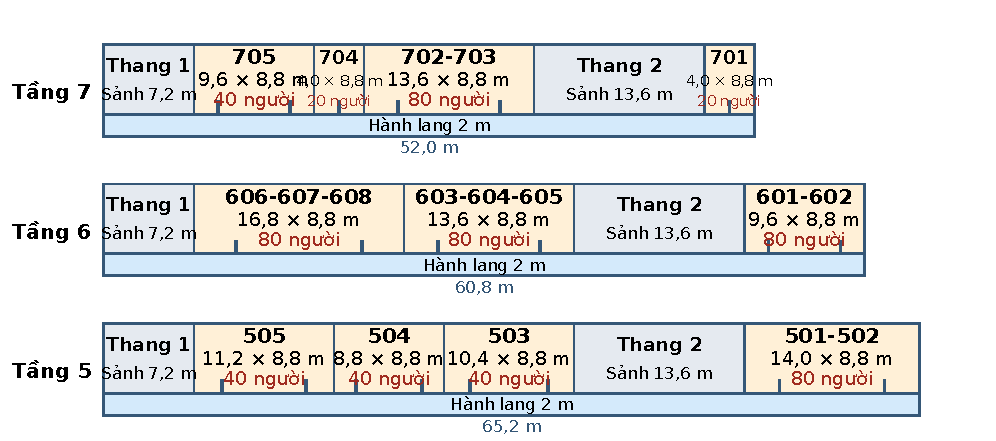
\includegraphics[width=\linewidth]{figures/a4_upper.pdf}
\caption{Các tầng 7--5.}\end{subfigure}
\begin{subfigure}{\linewidth}\centering
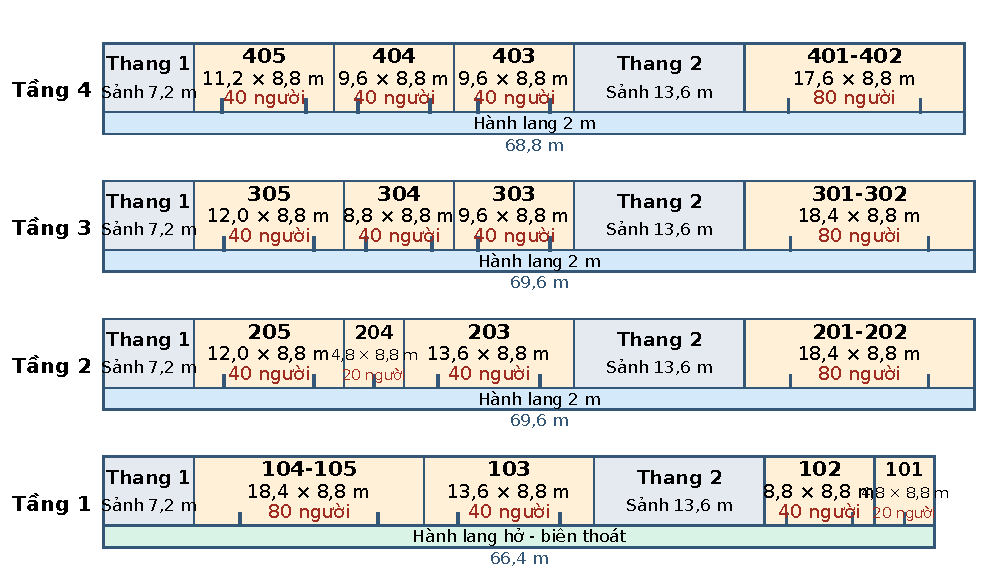
\includegraphics[width=\linewidth]{figures/a4_lower.pdf}
\caption{Các tầng 4--1.}\end{subfigure}
\caption{Mặt bằng tính toán của tòa nhà A4; dữ liệu chi tiết các khu phòng được trình bày tại phụ lục A.}
\label{fig:a4}\end{figure}
Tọa độ cục bộ từng tầng bảo toàn thứ tự và kích thước các khối. Các nút thang cùng chỉ số ở hai tầng kế tiếp được nối bằng quãng đường giữa tầng giả định.

\topic{Phạm vi mô hình và phân loại dữ liệu}
Đơn vị nguồn dân số là khu phòng có nhãn độc lập trong dữ liệu. Các nhãn ghép như 104-105 hoặc 603-604-605 được biểu diễn bởi một nguồn duy nhất với sức chứa của toàn khu. Quy tắc này bảo toàn tổng dân số khi chuyển mặt bằng thành đồ thị, đồng thời tránh đếm lặp các phần của một không gian đã gộp.

\bang{floors}{Đặc trưng hình học và sức chứa theo tầng}

Miền tính toán gồm phòng, cửa phòng, hành lang, sảnh và hai cụm cầu thang. Khu vệ sinh gần cụm thang 2 bị loại khỏi miền: không gán dân số, không tạo đường đi xuyên và không bổ sung diện tích chứa cho sảnh. Các sảnh tiếp cận thang được giữ như những vị trí trung chuyển riêng. Mạng di chuyển chỉ xét phương án sử dụng cầu thang bộ.

Dữ liệu đầu vào được phân thành ba thành phần: đặc trưng mặt bằng và sức chứa; điều kiện biên thoát tại hành lang hở tầng 1; và các tham số động lực học giả định. Thành phần thứ ba gồm bề rộng thông thủy cửa, bề rộng sử dụng vế thang, tốc độ di chuyển, suất thông hành và sức chứa tại các nút. Phân loại này phân biệt đặc trưng hình học với tham số cần hiệu chỉnh thực nghiệm.

Kích thước lõi thang 5 m trong sơ đồ được sử dụng để mô tả hình học. Khả năng thông hành trên thang được tính với bề rộng sử dụng giả định 1,5 m. Hai đại lượng có ngữ nghĩa khác nhau và được lưu riêng để bảo đảm khả năng kiểm soát cấu hình.

\topic{Yêu cầu hệ thống và tiêu chí đánh giá}
Mã nguồn và cấu hình thực nghiệm được công bố tại kho GitHub của nghiên cứu \cite{code}. Hệ thống được triển khai dưới dạng giao diện dòng lệnh, có chức năng sinh dữ liệu, giải lịch, kiểm tra độc lập và xuất kết quả. Mỗi lượt thực nghiệm lưu ảnh chụp mô hình, phân bố dân số, kịch bản nguy cơ, seed, phiên bản phần mềm và lịch hành động. Trực quan hóa được suy xuất từ lịch đã kiểm chứng để duy trì tính nhất quán với nghiệm tối ưu.

\begin{table}[htbp]\centering\caption{Các điều kiện kiểm chứng của hệ thống}
\small\begin{tabularx}{\linewidth}{P{1cm}P{4cm}X}\toprule
Mã & Điều kiện & Tiêu chí kiểm chứng\\\midrule
R1 & Nhất quán dữ liệu mặt bằng & 7 tầng, 27 khu phòng, 1.360 người; khu 705 có 40 người.\\
R2 & Đúng điều kiện biên & 7 cửa phòng tầng 1 và 2 vùng thoát từ sảnh thang.\\
R3 & Khả thi về năng lực & Lưu lượng cạnh và lượng chứa nút không vượt giới hạn.\\
R4 & Khả thi về thời gian & Mọi hành động kết thúc trước thời điểm mất an toàn.\\
R5 & Bảo toàn dân số & Tổng ở nút, đang đi, đã thoát và phơi nhiễm bằng đầu vào.\\
R6 & Khả năng tái lập & Lưu đủ cấu hình, lịch và kết quả kiểm tra.\\\bottomrule
\end{tabularx}\end{table}

Tiêu chí được áp dụng theo thứ tự ưu tiên: lượng người thoát; thời điểm thoát cuối của lượng này; và tổng thời điểm thoát. Thời gian trung bình được báo cáo đồng thời với số người thoát để tránh sai lệch diễn giải khi các phương pháp có tỷ lệ hoàn tất khác nhau.

Các giới hạn về dữ liệu, hành vi và thông tin nguy cơ được tổng hợp tại mục 5.8.

\topic{Tổng quan nghiên cứu và vị trí của mô hình}
Ford và Fulkerson \cite{ford} xét bài toán cực đại hóa lượng vận chuyển trong một khoảng thời gian khi mỗi cạnh có thời lượng và năng lực. Điểm cốt lõi là năng lực được khai thác lặp theo thời gian, vì vậy luồng tĩnh riêng lẻ chưa mô tả được lịch khởi hành. Mạng TEN sử dụng trong nghiên cứu kế thừa cách gắn thời gian vào trạng thái, đồng thời bổ sung sức chứa nút và mốc mất an toàn.

Chalmet, Francis và Saunders \cite{chalmet} xây dựng các mô hình mạng cho sơ tán công trình, liên kết cách biểu diễn không gian với số người thoát và thời điểm thoát. Tổng quan của Dhamala \cite{survey} phân biệt các lớp luồng cực đại, luồng chi phí nhỏ nhất, luồng nhanh nhất và luồng đến sớm. M4 sử dụng thứ tự ưu tiên về lượng thoát, thời điểm thoát cuối và tổng thời điểm thoát; việc tối ưu tổng thời điểm không đồng nghĩa tối ưu mọi tiền tố của đường cong tích lũy.

Các cấu trúc mạng dư, luồng cực đại và chi phí giảm được hệ thống hóa trong Ahuja, Magnanti và Orlin \cite{ahuja}. Trong bài toán A4, mạng dư phục vụ hiệu chỉnh phân bổ giữa nhiều nguồn phòng; potentials cho phép dùng đường ngắn nhất khi cạnh ngược xuất hiện chi phí âm. Sự kết hợp này tạo một mô hình điều phối thay vì ghép độc lập các tuyến ngắn nhất.

Khác biệt của trường hợp nghiên cứu là bảy cửa phòng tầng 1 kết thúc trực tiếp ở biên ngoài, trong khi dân số tầng trên phải qua hai hệ thang. Do đó, dân số tầng 1 không được cộng vào lưu lượng bắt buộc qua lát cắt cầu thang. Phân biệt này được sử dụng khi xây dựng cận dưới và phân tích nút thắt ở phần thực nghiệm.

\topic{Bố cục báo cáo và kế hoạch phân công}
Phần 1 xác lập bài toán và dữ liệu. Phần 2 trình bày đồ thị, ràng buộc và hàm mục tiêu. Phần 3 mô tả các thuật toán cùng lập luận tính đúng đắn. Phần 4 trình bày cài đặt và kiểm chứng. Phần 5 phân tích kết quả, đối chứng bổ sung, độ nhạy và giới hạn. Các phụ lục lưu danh sách khu phòng, ký hiệu và dấu vết dữ liệu.

\begin{table}[htbp]\centering\caption{Kế hoạch phân công nhiệm vụ trong nhóm}
\small\begin{tabularx}{\linewidth}{P{3cm}X}\toprule
Thành viên & Phạm vi phụ trách\\\midrule
Lý Thành Đạt & Tích hợp mô hình đồ thị, bộ tối ưu M4 và kiểm tra tính nhất quán của kết quả.\\
Đinh Đức Mạnh & Chuẩn hóa dữ liệu mặt bằng, mô hình nguy cơ và các phương pháp đối chứng.\\
Phạm Văn Đạt & Thiết kế thực nghiệm, trực quan hóa, tổng hợp bảng và biên tập nội dung.\\\bottomrule
\end{tabularx}\end{table}
Đây là kế hoạch phân công; việc rà soát số liệu và kết luận được thực hiện chung.
\clearpage\section{MÔ HÌNH ĐỒ THỊ VÀ MẠNG THỜI GIAN}
\subsection{Đồ thị không gian và ngữ nghĩa của các nút}
Đặt $G=(V,E)$ là đồ thị có hướng. Mỗi cạnh biểu diễn một thao tác đi từ một khu vực sang khu vực tiếp theo; hướng cạnh là hướng người có thể đi trong mô hình. Mỗi khu phòng chỉ có cạnh đi ra, nên không có tuyến dùng phòng đang có người như một lối xuyên hành lang.

\noindent\begin{minipage}[t]{0.45\linewidth}\begin{center}\small
\begin{tabular}{lr}
\toprule
Loại nút & Số lượng\\\midrule
CORRIDOR & 55\\
DOOR & 43\\
EXIT & 9\\
LOBBY & 14\\
ROOM & 27\\
STAIR & 14\\
\bottomrule\end{tabular}\end{center}\end{minipage}\hfill
\begin{minipage}[t]{0.53\linewidth}\begin{center}\small
\begin{tabular}{lr}
\toprule
Loại cạnh có hướng & Số lượng\\\midrule
CORE\_ACCESS & 54\\
CORRIDOR\_LANE & 98\\
DOOR\_CORRIDOR & 43\\
ROOM\_DOOR & 50\\
STAIR\_DOWN & 12\\
\bottomrule\end{tabular}\end{center}\end{minipage}

Đồ thị được sinh có 162 nút và 257 cạnh có hướng. ROOM là nơi xuất phát; DOOR là cửa phòng tầng trên; CORRIDOR là vị trí trên hành lang; LOBBY là sảnh tiếp cận thang; STAIR là nút trên cụm thang; EXIT là biên kết thúc sơ tán. Có 43 nút DOOR ở tầng 2--7 và bảy cửa phòng tầng 1 mang trực tiếp loại EXIT.

Quy tắc biểu diễn cửa dựa trên chú giải mặt bằng: khu ghép và phòng có chiều dài từ 8 m được gán hai cửa; phòng ngắn hơn được gán một cửa. Hai cửa có tọa độ quy ước tại 20\% và 80\% chiều dài. Khoảng cách từ tâm phòng đến cửa được tính trong hệ cục bộ, biểu diễn phần di chuyển bên trong phòng trước khi tiếp cận biên cửa.

Cạnh thang nối hai tầng kề theo hướng đi xuống và giữ chỉ số cụm thang. Thời lượng được tính từ quãng đường giữa tầng giả định, độc lập với tọa độ ngang cục bộ.

\topic{Điều kiện thoát tại hành lang hở tầng 1}
Điều kiện biên ở tầng 1 là hành lang hở có khả năng tiếp cận trực tiếp không gian ngoài. Với cửa phòng tầng 1 ký hiệu $D$, thời điểm thoát được xác định bởi
\begin{equation}T_{\mathrm{exit}}=T_{\mathrm{arrival}}(D).\end{equation}
Sự kiện thoát trùng với thời điểm đến cửa. Thời lượng tiếp cận cửa từ trong phòng và năng lực thông hành của cửa vẫn tham gia các ràng buộc; không phát sinh thao tác chuyển tiếp sau biên này.

\hinh{ground_vector.pdf}{Bảy cửa phòng tầng 1 và hai vùng thoát từ sảnh thang.}

Mỗi cửa phòng tầng 1 có năng lực hấp thụ bằng năng lực của chính cửa đó. Với bề rộng giả định 1,2 m, suất thông hành 1,3 người/(m.s) và bước 5 s, mỗi cửa cho vào tối đa $\lfloor1{,}2\times1{,}3\times5\rfloor=7$ người/bước. Phòng 101 có 20 người, nên có thể xuất hiện ba đoàn 7, 7 và 6 người; việc coi hành lang là vùng ngoài không làm mất hàng đợi này.

Người ở tầng trên đi xuống thang, qua sảnh tầng 1 rồi tới hành lang hở. Hai nhãn EXIT1 và EXIT2 chỉ hai vùng tiếp cận đó, không phải hai cửa vật lý bổ sung. Năng lực hấp thụ tại mỗi vùng đặt bằng $N=1.360$ để không tạo thêm nút thắt; lưu lượng thực đã bị giới hạn bởi cạnh tiếp cận sảnh và thang.

EXIT là nút hấp thụ, không có cạnh người đi ra hoặc hành động chờ tại đó.

\topic{Rời rạc hóa thời gian và giả định năng lực}
Mô hình dùng các mốc $t_k=k\Delta t$. Với cạnh $e$ dài $\ell_e$, tốc độ $v_e$, số bước đi là $d_e=\max(1,\lceil\ell_e/(v_e\Delta t)\rceil)$. Phép làm tròn lên giúp tránh đến sớm hơn thời lượng liên tục đã giả định, nhưng tạo sai khác tích lũy trên tuyến nhiều cạnh.

\begin{table}[htbp]\centering\caption{Cấu hình tham số cơ sở và phân loại nguồn}
\small\begin{tabularx}{\linewidth}{P{5.1cm}P{2.7cm}X}\toprule
Tham số & Giá trị & Nguồn / loại tham số\\\midrule
Bước thời gian & 5 s & Thiết kế rời rạc hóa.\\
Tốc độ đi bộ / trên thang & 1,2 / 0,7 m/s & Minh họa, cần hiệu chỉnh.\\
Quãng đường giữa hai tầng & 12 m & Giả định hình học.\\
Suất thông hành $q$ & 1,3 người/(m.s) & Minh họa, không phải số đo A4.\\
Bề rộng cửa phòng & 1,2 m & Giả định thông thủy.\\
Bề rộng sử dụng vế thang & 1,5 m & Giả định, khác lõi thang 5 m.\\
Bề rộng hành lang / làn & 2 / 1 m & Sơ đồ / quy tắc chia làn.\\
Sức chứa nút hành lang & 24 người & Minh họa ở mức nút.\\
Sức chứa sảnh / thang & 30 / 36 người & Minh họa ở mức nút.\\
Lan cháy / khói ngang & 0,03 / 0,15 m/s & Độ trễ sự kiện minh họa.\\
Khói lên / xuống một tầng & 25 / 45 s & Độ trễ sự kiện minh họa.\\\bottomrule
\end{tabularx}\end{table}

Năng lực khởi hành của cạnh có bề rộng $w_e$ là $U_e=\lfloor w_eq\Delta t\rfloor$. Hành lang 2 m được chia cố định thành hai làn 1 m, mỗi chiều một làn. Cách này tránh cấp đồng thời toàn bộ 2 m cho cả hai hướng, nhưng chưa tối ưu việc chia sẻ bề rộng linh hoạt.

Sức chứa đang đi được xác lập theo mô hình đoàn, $C_e=d_eU_e$, tương ứng tối đa $d_e$ đoàn khởi hành đồng thời hiện diện trên cạnh. Cấu hình này bảo đảm ràng buộc tổng đang đi từ năng lực từng bước. Trường hợp $C_e<d_eU_e$ đòi hỏi thêm ràng buộc chiếm dụng chồng lấp và nằm ngoài miền cấu hình được bộ giải chấp nhận.

\topic{Xây dựng mạng mở rộng theo thời gian}
Với horizon $K$, mỗi trạng thái hợp lệ $(v,k)$ được tách thành hai nút $(v,k)^{\mathrm{in}}$ và $(v,k)^{\mathrm{out}}$. Cạnh nối hai nút có dung lượng $B_v$, nhờ đó mọi người hiện diện ở cùng vị trí và mốc thời gian phải cùng đi qua một giới hạn chứa.

\begin{figure}[htbp]\centering
\begin{tikzpicture}[>=Stealth,node distance=1.8cm,every node/.style={font=\small}]
\node[draw,rounded corners] (ui) {$u_k^{\mathrm{in}}$};
\node[draw,rounded corners,right=of ui] (uo) {$u_k^{\mathrm{out}}$};
\node[draw,rounded corners,right=2.8cm of uo] (vi) {$v_{k+d}^{\mathrm{in}}$};
\node[draw,rounded corners,below=1.7cm of ui] (un) {$u_{k+1}^{\mathrm{in}}$};
\draw[->,thick] (ui)--node[above,align=center]{Tách nút\\$B_u$}(uo);
\draw[->,thick] (uo)--node[above,align=center]{Di chuyển\\$U_e$, $d_e$ bước}(vi);
\draw[->,thick] (uo)--node[below right,align=center]{Chờ một bước\\$B_u$}(un);
\end{tikzpicture}
\caption{Tách nút, cạnh di chuyển và cạnh chờ trong TEN.}\end{figure}

Gọi $x_{e,k}$ là số người bắt đầu cạnh $e$ ở bước $k$, $z_{v,k}$ là số người chờ sang bước kế tiếp và $y_{v,k}$ là lượng hiện diện. Các giới hạn chính gồm
\begin{align}0\le x_{e,k}\le U_e,\quad 0\le y_{v,k}\le B_v,\\
\text{tổng đến tại }(v,k)=\text{tổng đi hoặc chờ từ }(v,k).
\end{align}
Siêu nguồn cấp dân số phòng ở bước 0; mỗi EXIT nối siêu đích tại đúng bước đến. Chỉ tạo cạnh chờ nếu vị trí cho chờ và cả hai mốc đều an toàn. Cạnh đi nối bước $k$ tới $k+d_e$, vì vậy thời gian không bị bỏ qua khi tối ưu luồng.

Do mọi dung lượng nguyên, luồng có thể phân rã thành nhóm nguyên. Không cần làm tròn một nghiệm phân số sau tối ưu, nhờ đó tránh tạo thêm vi phạm năng lực do bước hậu xử lý.

\topic{Lịch nguy cơ và ranh giới an toàn}
Cháy và khói được mô hình hóa bằng các thời điểm sự kiện trên đồ thị. Một hoặc nhiều nguồn có thời điểm bắt đầu; Dijkstra đa nguồn lan truyền thời điểm sớm nhất tới các vị trí còn lại. Đồ thị nguy cơ khác đồ thị người đi: khói có thể lan lên thang, dù người trong mô hình chỉ đi xuống.

Tại nút $v$, thời điểm mất an toàn là
\begin{equation}T_v=\min(T_v^{fire},T_v^{smoke},T_v^{closure}).\end{equation}
Điều kiện hợp lệ là $t<T_v$, không phải $t\le T_v$. Ví dụ, một vùng bị chặn ở 120 s vẫn hợp lệ tại 119,999 s nhưng không hợp lệ tại 120 s. Quy ước này được kiểm tra bằng ca thử riêng để tránh sai khác ở đúng mốc nguy hiểm.

\begin{table}[htbp]\centering\caption{Ví dụ kiểm tra một cạnh có mốc đóng 120 s}
\small\begin{tabular}{rrl}\toprule Khởi hành & Đến & Kết luận\\\midrule
100 s & 115 s & Có thể hợp lệ nếu hai đầu an toàn.\\
105 s & 120 s & Không hợp lệ: đến đúng mốc đóng.\\
115 s & 130 s & Không hợp lệ: chuyến đi vượt mốc.\\\bottomrule\end{tabular}\end{table}

Cạnh bị đóng bảo thủ khi một trong hai đầu không an toàn hoặc đến mốc khóa cạnh riêng. Toàn bộ chuyến đi phải kết thúc trước mốc đóng của cạnh. Do đó, chỉ kiểm tra an toàn lúc khởi hành là không đủ: người có thể đang trên đường khi khói tới.

Lịch nguy cơ được xác định trước trong toàn bộ horizon. Đây là bài toán tối ưu ngoại tuyến với thông tin hoàn hảo; các tham số lan truyền biểu diễn độ trễ sự kiện trên mạng.

\topic{Mục tiêu ưu tiên và tính đơn điệu theo horizon}
Gọi $F(K)$ là max flow trên TEN đến bước $K$. Đầu tiên tính $F^*=F(K_{max})$ để xác định số người tối đa có thể sơ tán trong thời hạn. Sau đó tìm horizon nhỏ nhất vẫn sơ tán được lượng này:
\begin{equation}K^*=\min\{K:F(K)\ge F^*\}.\end{equation}
Ở $K^*$, bài toán luồng chi phí nhỏ nhất gửi đúng $F^*$ người, với chi phí trên cạnh thoát ở bước $k$ bằng $k$. Mục tiêu cuối là $\min\sum_{v\in EXIT,k}k f_{v,k}$.

\begin{dinhly}Với lịch nguy cơ cố định và mô hình hiện tại, $F(K)$ không giảm khi tăng $K$.\end{dinhly}
\begin{proof}
Mọi hành động của một lịch đến hạn $K$ vẫn nằm trong hạn $K+1$ và có cùng thời điểm nguy hiểm, năng lực và thời lượng. Người đã thoát trước $K$ không phải chờ thêm. Phép cắt theo cận dưới cũng không loại trạng thái đã hợp lệ khi horizon tăng. Vì vậy lịch cũ vẫn là ứng viên của bài toán mới, nên giá trị max flow không thể nhỏ hơn.
\end{proof}

Tính đơn điệu cho phép tìm kiếm nhị phân. Nếu $F^*<N$, vẫn tìm được thời điểm thoát cuối cho lượng thoát tối đa, nhưng không gọi đó là makespan hoàn tất toàn dân số. Trường hợp này được báo là chưa hoàn tất và giữ makespan toàn dân số ở giá trị thiếu.

Mục tiêu ba cấp xác định quan hệ ưu tiên từ điển giữa lượng thoát, thời hạn và tổng thời điểm thoát. Việc tối ưu tổng chi phí chỉ được thực hiện sau khi cố định hai mục tiêu trước, nên không xảy ra đánh đổi lượng người thoát để giảm tổng thời gian của một tập dân số nhỏ hơn.

\topic{Ví dụ tính tay và giới hạn chứa theo đoàn}
Xét một nguồn 10 người có hai tuyến đến vùng ngoài. Tuyến A đi mất 2 bước, cho vào tối đa 3 người/bước; tuyến B đi mất 3 bước, cho vào tối đa 2 người/bước. Bỏ qua giới hạn nút trung gian trong ví dụ để tách riêng tác động thời lượng và năng lực.

\begin{table}[htbp]\centering\caption{Một lịch sơ tán đủ 10 người cho ví dụ hai tuyến}
\small\begin{tabular}{crrrr}\toprule Bước khởi hành & Vào A & Bước đến A & Vào B & Bước đến B\\\midrule
0 & 3 & 2 & 2 & 3\\1 & 3 & 3 & 2 & 4\\\bottomrule\end{tabular}\end{table}
Đến hết bước 2 chỉ ba người tới đích. Đến hết bước 3 có thể đưa thêm ba người theo A và hai người từ B khởi hành ở bước 0, đạt tám người. Muốn sơ tán đủ mười trước hoặc tại bước 3 là không thể vì các suất vào còn lại chưa kịp tới đích. Lịch trên hoàn tất ở bước 4; tổng thời điểm thoát là $3\cdot2+3\cdot3+2\cdot3+2\cdot4=29$ đơn vị bước.

Với cạnh A, có hai đoàn khởi hành chồng lấp, mỗi đoàn tối đa ba người. Sức chứa đang đi $C_A=2\times3=6$ là hệ quả của cách đặt năng lực. Tổng quát,
\begin{equation}\sum_{j=k-d_e+1}^{k}x_{e,j}\le d_eU_e=C_e.\end{equation}
Trong cấu hình đoàn, bất đẳng thức bảo đảm tổng người đang đi thông qua các giới hạn khởi hành. Nếu $C_A=4$ trong khi $U_A=3$, cận $d_AU_A=6$ không bảo đảm ràng buộc chứa 4. Trường hợp đó yêu cầu biểu diễn tài nguyên chồng lấp trong mô hình, thay vì chỉ hiệu chỉnh một thuộc tính dữ liệu.

Ví dụ minh họa cơ chế ràng buộc; kết quả A4 được trình bày ở phần 5.
\clearpage\section{THIẾT KẾ VÀ PHÂN TÍCH THUẬT TOÁN}
\subsection{Dijkstra và vai trò giới hạn của A*}
Dijkstra tìm đường có tổng trọng số nhỏ nhất khi trọng số không âm \cite{dijkstra}. Trong chương trình, đồ thị tìm tuyến dùng thời lượng cạnh theo bước; nhãn khoảng cách lưu chi phí tốt nhất hiện biết và hàng đợi ưu tiên chọn nhãn nhỏ nhất để mở rộng. Mỗi bản ghi cha lưu cả đỉnh trước và mã cạnh, nhờ đó có thể khôi phục một tuyến gồm các cạnh xác định.

\begin{algorithm}[htbp]\caption{Tìm tuyến ngắn nhất tới một tập đích}\label{alg:1}
\begin{lstlisting}[frame=none]
DIJKSTRA(G, source, exits):
    dist[source] = 0; heap = [(0, source)]
    while heap is not empty:
        (d,u) = pop_min(heap)
        if d != dist[u]: continue
        if u in exits: return reconstruct(parent,u)
        for edge (u,v,w) in G[u]:
            if d+w < dist[v]:
                dist[v] = d+w
                parent[v] = (u, edge.id)
                push(heap,(dist[v],v))
    return NO_PATH
\end{lstlisting}
\end{algorithm}
Một đỉnh có thể có nhiều bản ghi trong heap. Bản ghi cũ bị bỏ bằng phép so sánh với nhãn hiện tại, tránh phải cài đặt thao tác giảm khóa. Cách này đơn giản và vẫn giữ giới hạn chuẩn theo số lần nới lỏng thành công.

Giao diện hỗ trợ A* với heuristic không vượt chi phí còn lại và bằng 0 tại đích. Thực nghiệm dùng $h=0$, tương ứng Dijkstra; A* được kiểm thử ở mức hàm.

Bài toán đường đi đơn tối ưu tổng trọng số mà chưa phân bổ năng lực giữa các nguồn. Trong M1--M3, tuyến được kết hợp với bộ kiểm tra sức chứa khi cam kết hành động. Sự phân tách giữa lựa chọn tuyến và khả năng phục vụ là cơ sở phân biệt các đối chứng cục bộ với mô hình điều phối toàn cục.

\topic{Dijkstra đa nguồn và tuyến phụ thuộc thời điểm}
Thời điểm nguy cơ đến các nút được xác định bằng khởi tạo đa nguồn. Heap chứa toàn bộ nguồn sự cố cùng mốc bắt đầu tương ứng; mỗi nhãn nút giữ thời điểm đến nhỏ nhất. Một nguồn khởi phát muộn vẫn có thể quyết định nhãn của vùng lân cận khi độ trễ truyền từ các nguồn khác lớn hơn.

\begin{algorithm}[htbp]\caption{Lan truyền thời điểm sự kiện}\label{alg:2}
\begin{lstlisting}[frame=none]
PROPAGATE(graph, sources):
    time[v] = infinity for all v
    for (v,start) in sources:
        if start < time[v]:
            time[v] = start; push(heap,(start,v))
    while heap is not empty:
        (t,u) = pop_min(heap)
        if t != time[u]: continue
        for (v,delay) in graph[u]:
            if t+delay < time[v]:
                time[v] = t+delay
                push(heap,(time[v],v))
    return time
\end{lstlisting}
\end{algorithm}
Với độ trễ $a\to b$ bằng 10 s và $b\to c$ bằng 5 s, hai nguồn bắt đầu tại $a$ lúc 20 s và tại $b$ lúc 7 s cho nhãn $c$ bằng 12 s. Nguồn $b$ xác lập nhãn sớm hơn giá trị 35 s truyền từ $a$. Cấu hình này được sử dụng như một ca kiểm thử xác định của hàm đa nguồn.

Hàm tìm đường an toàn dùng nhãn là bước đến tuyệt đối. Khi xét cạnh từ $u$ ở bước $k$, nó tính $k+d_e$ rồi kiểm tra an toàn lúc đến và trong chuyến đi. Việc đến sớm hơn là không bất lợi trong mô hình có mốc đóng đơn điệu: không có cửa mở lại hoặc lợi ích do cố ý đến muộn để bắt một khoảng mở tương lai.

Kết quả của hàm vẫn chưa xét hàng đợi. M2 gọi lại hàm tại vị trí hiện tại, trong khi M4 đưa cả nguy cơ lẫn năng lực vào cùng một mạng thời gian để điều phối toàn cục.

\topic{Dinic, mạng dư và luồng cực đại}
Thuật toán Dinic \cite{dinic} sử dụng đồ thị mức và luồng chặn. Mỗi cạnh thuận có một cạnh dư ngược tương ứng. Phép tăng $a$ đơn vị làm giảm dung lượng dư thuận và tăng dung lượng dư ngược cùng lượng $a$. Cấu trúc này cho phép hiệu chỉnh phân bổ luồng đã thiết lập ở các pha trước trong khi vẫn bảo toàn điều kiện cân bằng.

\begin{algorithm}[htbp]\caption{Giải luồng cực đại bằng Dinic}\label{alg:3}
\begin{lstlisting}[frame=none]
DINIC(network,s,t,limit):
    flow = 0
    while flow < limit:
        level = BFS_on_positive_residual_arcs(s)
        if t is unreachable: break
        pointer[v] = 0 for every v
        while an admissible s-t path exists:
            path = iterative_DFS_using_level_and_pointer()
            a = min(limit-flow, bottleneck(path))
            push_on_path_and_reverse_arcs(path,a)
            flow += a
    return flow
\end{lstlisting}
\end{algorithm}
BFS xây đồ thị mức; DFS chỉ đi sang mức kế tiếp. Mỗi đỉnh có con trỏ để không quét lại những cạnh đã xác định không còn dùng được trong pha. Khi không tăng được trong đồ thị mức, thuật toán dựng mức mới trên mạng dư hiện tại.

DFS được viết lặp bằng stack. Điều này có ý nghĩa vì mạng thời gian có thể chứa đường đi dài hơn độ sâu đệ quy mặc định. Ca kiểm thử chuỗi 2.100 cạnh với năng lực 3 xác nhận chương trình không phụ thuộc tăng giới hạn đệ quy.

Trên TEN đến hạn $K$, một đơn vị luồng tương ứng một người có chuỗi hành động hợp lệ. Khi không còn đường tăng, lượng gửi là luồng cực đại của mạng đã dựng.

\topic{Min-Cost Flow với potentials và blocking flow}
Sau khi cố định lượng cần gửi, cần chọn lịch có tổng thời điểm thoát nhỏ nhất. Cạnh thuận ban đầu có chi phí không âm, nhưng cạnh dư ngược có chi phí đối dấu. Vì vậy, không thể chạy Dijkstra trực tiếp trên chi phí gốc sau mọi lần tăng luồng.

Phương pháp sử dụng potentials $p$ và chi phí giảm $c^{\prime}(u,v)=c(u,v)+p(u)-p(v)$ trong bài toán luồng chi phí nhỏ nhất \cite{mitflow}. Tính nhất quán của triển khai được đối chiếu với bộ giải tham chiếu trên các đồ thị nguyên quy mô nhỏ.
\begin{algorithm}[htbp]\caption{Luồng chi phí nhỏ nhất với potentials và luồng chặn}\label{alg:4}
\begin{lstlisting}[frame=none]
MIN_COST(net,s,t,required):
    potential[v] = 0; flow = cost = 0
    while flow < required:
        dist = DIJKSTRA_RESIDUAL(reduced_cost)
        if dist[t] is infinity: break
        for every reachable v:
            potential[v] += dist[v]
        a = DINIC_ON_ZERO_REDUCED_COST_ARCS(
                s,t,required-flow)
        cost += a*(potential[t]-potential[s])
        flow += a
    return flow,cost
\end{lstlisting}
\end{algorithm}
Sau khi cập nhật potentials, mọi đường nguồn--đích chỉ gồm cạnh có chi phí giảm 0 có cùng chi phí gốc $p(t)-p(s)$. Thay vì chạy heap riêng cho từng nhóm nhỏ, chương trình gửi một blocking flow trên tập cạnh này và tính chi phí theo tổng lượng gửi được.

Điều kiện đầu vào của hàm là chi phí thuận ban đầu không âm. Các cạnh ngược âm sinh trong mạng dư vẫn được phép; chương trình không tuyên bố hỗ trợ mọi mạng có chi phí âm ban đầu. Trong TEN, chi phí chỉ đặt ở cạnh thoát và bằng bước $k$, nên điều kiện khởi tạo potentials bằng 0 được thỏa mãn.

\topic{Quy trình tối ưu M4 và cắt trạng thái hợp lệ}
Quy trình M4 gồm ba giai đoạn liên tiếp: xác định lượng thoát tối đa, tìm horizon tối thiểu và tối ưu tổng thời điểm thoát. Mạng ở giai đoạn cuối được dựng độc lập với các phép dò trước để khởi tạo đúng dung lượng dư và chi phí tại horizon đã xác lập.
\begin{algorithm}[htbp]\caption{Tối ưu ba mục tiêu M4 trên TEN}\label{alg:5}
\begin{lstlisting}[frame=none]
OPTIMIZE(building,hazards,occupancy,Kmax):
    lower = reverse_shortest_distance_to_any_exit()
    F = DINIC(TEN(Kmax,lower))
    lo = 0; hi = Kmax
    while lo < hi:
        mid = floor((lo+hi)/2)
        if DINIC(TEN(mid,lower)) >= F: hi = mid
        else: lo = mid+1
    net = TEN(lo,lower)
    (value,cost) = MIN_COST(net,F)
    assert value == F
    schedule = DECOMPOSE(net)
    assert VALIDATE(schedule)
    return schedule
\end{lstlisting}
\end{algorithm}
Cận dưới $\operatorname{lower}(v)$ là thời gian tới một EXIT khi bỏ qua hàng đợi và nguy cơ. Trạng thái $(v,k)$ bị cắt nếu $k+\operatorname{lower}(v)>K$. Một người không thể đi nhanh hơn đường tự do, nên phép cắt không loại lịch khả thi; nó chỉ tránh tạo trạng thái đã chắc chắn không kịp ra ngoài.

\bang{probes}{Các lần dò max flow thực tế của M4, không sự cố}

Bảng ghi các phép dò horizon: thời hạn 900 s tương ứng 180 bước; horizon hoàn tất tối ưu là 78 bước, tức 390 s.

\topic{Phân rã luồng và lập luận bảo toàn ràng buộc}
Mạng thuận tiến theo thời gian nên không có chu trình thời gian trong phần luồng dương được phân rã. Từ siêu nguồn, chọn các cạnh còn luồng đến siêu đích, lấy lượng nhỏ nhất trên đường làm kích thước nhóm, rồi trừ lượng đó khỏi các cạnh đã đi. Lặp lại đến khi không còn luồng từ nguồn.

\begin{table}[htbp]\centering\caption{Ánh xạ thành phần mạng sang lịch hành động}
\small\begin{tabularx}{\linewidth}{P{4cm}X}\toprule
Thành phần mạng & Bản ghi sau giải mã\\\midrule
Cạnh siêu nguồn--phòng & Nguồn của nhóm và số người.\\
Cạnh nối hai mốc cùng nút & WAIT, từ bước $k$ tới $k+1$.\\
Cạnh đi $u_k\to v_{k+d}$ & MOVE, mã cạnh và mốc đi/đến.\\
Cạnh EXIT--siêu đích & Điểm thoát và bước thoát.\\\bottomrule
\end{tabularx}\end{table}

\begin{dinhly}Mỗi đường luồng đã giải mã tôn trọng giới hạn thời lượng và năng lực của TEN.\end{dinhly}
\begin{proof}
Mỗi cạnh di chuyển nối đúng hai mốc cách nhau $d_e$, nên thời lượng của MOVE đúng bằng số bước cạnh. Mọi lượng đi qua cạnh đó không vượt dung lượng $U_e$. Mọi lượng hiện diện tại cùng trạng thái đi qua cạnh tách nút dung lượng $B_v$. Phân rã chỉ chia luồng thành các đường và không làm tăng tổng luồng trên bất kỳ cạnh nào, vì vậy các giới hạn tiếp tục được giữ.
\end{proof}

Ngoài các bất biến của luồng, quá trình chuyển đổi nghiệm cần kiểm chứng metadata thời gian và sự kiện thoát. Bộ kiểm tra độc lập dựng lại mức sử dụng tài nguyên từ lịch hành động sau phân rã. Cách tiếp cận này tách bằng chứng khả thi của lịch khỏi cấu trúc dữ liệu mạng dư của bộ giải.

Người không được chọn vào các đường sơ tán vẫn tồn tại tại nguồn. Phòng không có cạnh đi vào, nên số người ở lại không làm một luồng khác đi xuyên qua nguồn và chiếm chỗ sai. Khi nguồn mất an toàn, họ được báo phơi nhiễm riêng, không bị chuyển thành người đã thoát.

\topic{Các phương pháp đối chứng và chính sách chia tải}
M1--M4 có chung đồ thị, phân bố dân số, lịch nguy cơ và các giới hạn năng lực. Biến can thiệp trong so sánh là chiến lược lựa chọn tuyến và thời điểm cam kết di chuyển. Mọi phương pháp đều áp dụng cùng bộ kiểm tra khả thi và quy tắc ghi nhận phần dân số chưa thoát.

\begin{table}[htbp]\centering\caption{Quy tắc ra quyết định của các phương pháp}
\small\begin{tabularx}{\linewidth}{P{1cm}P{4.2cm}X}\toprule
PP & Chọn tuyến & Xử lý năng lực\\\midrule
M1 & Tuyến ngắn nhất ở thời điểm đầu, giữ cố định. & Chờ nếu cạnh kế tiếp không nhận được người.\\
M2 & Tính lại tuyến an toàn tại vị trí, thời điểm hiện tại. & Chọn bước đầu tuyến mới rồi kiểm tra chỗ.\\
M3 & Chấm điểm các bước khả thi và chọn tham lam. & Xét lượng đặt chỗ khi chấm điểm.\\
M4 & Điều phối toàn cục trên TEN. & Năng lực là dung lượng trong bài toán luồng.\\
M1E & Chia đều hai thang, giữ tuyến ngắn nhất đến đích đã gán. & Cùng chính sách đặt chỗ và chờ của M1.\\\bottomrule
\end{tabularx}\end{table}
Điểm M3 gồm thời lượng bước đang xét, thời gian đường còn lại và hai thành phần phạt tỷ lệ sử dụng cạnh, nút:
\begin{equation}\operatorname{score}(e,k)=d_e+\operatorname{lower}_{safe}(v,k+d_e)+\alpha\rho_e+\alpha\rho_v.\end{equation}
Ở đây $\rho_e$ là tỷ lệ năng lực cạnh đã đặt tại bước $k$; $\rho_v$ là tỷ lệ sức chứa nút đích đã đặt tại bước đến. Cấu hình chính dùng $\alpha=4$; khảo sát bổ sung xét $\alpha\in\{1,2,4,8\}$. M1E gán luân phiên từng người ở tầng trên cho EXIT1 và EXIT2, rồi tính tuyến ngắn nhất đến vùng thoát được gán; 180 người tầng 1 vẫn đi trực tiếp qua cửa phòng. Vì vậy, đối chứng này kiểm tra riêng lợi ích của cân bằng tải khi chưa tối ưu toàn cục.

Các baseline phá hòa theo ID nguồn/người và đặt chỗ bảo thủ ở nút cho đến khi có lệnh rời được cam kết. Chính sách này bảo đảm lịch kiểm tra được nhưng có thể làm giảm hiệu quả. Vì vậy, kết quả so sánh vừa phản ánh khả năng điều phối toàn cục, vừa phản ánh những quy tắc cụ thể của bộ đối chứng đang cài đặt.

\topic{Độ phức tạp, tính đúng đắn và giới hạn khẳng định}
Đặt $n=|V|$, $m=|E|$, horizon $K$ và số pha chi phí của Min-Cost Flow là $P$. Quy mô TEN trước cắt có bậc $O(nK)$ nút, $O((n+m)K)$ cạnh. Giảm $K$ hoặc cắt trạng thái có thể tiết kiệm đáng kể tài nguyên nhưng không làm thay đổi bản chất tăng theo thời gian của mô hình.

\begin{table}[htbp]\centering\caption{Các mức phân tích độ phức tạp}
\small\begin{tabularx}{\linewidth}{P{4cm}X}\toprule
Thành phần & Giới hạn và ý nghĩa\\\midrule
Dijkstra với heap & $O((n+m)\log n)$ theo cách biểu diễn đồ thị.\\
Dijkstra đa nguồn & Cùng bậc; thêm các nguồn vào khởi tạo.\\
Dinic tổng quát & $O((n^{\prime})^2m^{\prime})$ trên mạng có $n^{\prime},m^{\prime}$.\\
Dựng TEN & $O((n+m)K)$ trước các chi tiết truy cập.\\
Tìm horizon & $O(\log(K+1))$ lần dò max flow sau lần dò hạn cuối.\\
Min-Cost Flow & $P$ pha đường ngắn nhất và blocking flow; không đồng nhất với một lần Dinic.\\\bottomrule
\end{tabularx}\end{table}

Lập luận tính đúng đắn được tách thành các nghĩa vụ: đồ thị đúng dữ liệu; TEN đúng thời gian và năng lực; max flow cho lượng thoát tối đa; tính đơn điệu cho tìm kiếm nhị phân; chi phí cạnh thoát cho đúng mục tiêu; phân rã và validator giữ đúng lịch. Việc bỏ qua một nghĩa vụ có thể làm kết luận tổng thể sai dù một thuật toán con đã được cài đúng.

Cơ sở lý thuyết của các thuật toán đường đi và mạng luồng được trình bày trong \cite{clrs}. Mô hình đoàn, điều kiện biên tầng 1 và thiết kế đối chứng được xác lập riêng cho trường hợp A4. Độ phức tạp mô tả bậc tăng theo quy mô; thời gian giải và mức sử dụng bộ nhớ cần được xác định bằng phép đo trên môi trường thực nghiệm cụ thể.

\clearpage\section{CÀI ĐẶT VÀ KIỂM CHỨNG CHƯƠNG TRÌNH}
\subsection{Kiến trúc và luồng xử lý}
Kiến trúc phần mềm gồm các thành phần dữ liệu, nguy cơ, tối ưu, kiểm chứng và trực quan hóa. Bộ sinh A4 thiết lập đồ thị; mô-đun nguy cơ xác định các mốc đóng; bộ giải và bộ kiểm tra lần lượt tạo lịch và đánh giá tính khả thi. Thành phần trực quan hóa đọc kết quả đã lưu.

\begin{figure}[htbp]\centering
\begin{tikzpicture}[>=Stealth,every node/.style={font=\footnotesize,draw,rounded corners,align=center,minimum width=2.1cm,minimum height=1.1cm},node distance=.45cm]
\node (a) {Mặt bằng\\và tham số};
\node[right=of a] (b) {Đồ thị\\và nguy cơ};
\node[right=of b] (c) {Bộ giải\\M1--M4};
\node[right=of c] (d) {Lịch và\\kiểm chứng};
\node[right=of d] (e) {Chỉ số và\\phát lại};
\draw[->] (a)--(b);\draw[->] (b)--(c);\draw[->] (c)--(d);\draw[->] (d)--(e);
\end{tikzpicture}\caption{Luồng dữ liệu của chương trình CLI.}\end{figure}

\begin{table}[htbp]\centering\caption{Các mô-đun chính}
\small\begin{tabularx}{\linewidth}{P{4.5cm}X}\toprule
Tệp & Trách nhiệm\\\midrule
\texttt{data.py}, \texttt{hazards.py} & Nhập sơ đồ, lưu giả định, tính mốc nguy cơ.\\
\texttt{algorithms.py} & Dijkstra, đa nguồn, Dinic, Min-Cost Flow tự viết.\\
\texttt{optimize.py}, \texttt{baselines.py} & TEN, M4 và ba bộ đối chứng.\\
\texttt{schedule.py}, \texttt{runner.py} & Kiểm tra, phát lại, đo và xuất dữ liệu.\\
\texttt{visuals.py}, \texttt{cli.py} & Hiển thị và giao diện dòng lệnh.\\\bottomrule
\end{tabularx}\end{table}
Các thuật toán chính được cài đặt trong mô-đun nội bộ. NetworkX chỉ đóng vai trò tham chiếu trong kiểm thử đồ thị nhỏ.

\topic{Cấu trúc dữ liệu và hợp đồng đầu vào}
Các cấu trúc Node và Edge lưu thông tin đủ để solver và bộ phát lại cùng hiểu một hành động. Node có ID, tầng, tọa độ, loại, sức chứa, quyền chờ và năng lực thoát. Edge có hai đầu, chiều dài, thời gian, năng lực vào, sức chứa đang đi và loại cạnh. Mọi ID được lập chỉ mục để phát hiện trùng và tra cứu nhất quán.

\begin{lstlisting}
Node(id, floor, x, y, kind,
     storage_capacity, can_wait, exit_capacity)
Edge(id, source, target, length_m,
     travel_seconds, entry_capacity,
     in_transit_capacity, kind)
Action(kind, source, target, depart,
       arrive, edge_id)
Journey(id, source, count, actions,
        exit_node, exit_step)
\end{lstlisting}
Ràng buộc kiểu dữ liệu yêu cầu dân số là số nguyên không âm, không vượt sức chứa khu phòng và loại trừ kiểu logic. Các tham số thời gian, tốc độ phải hữu hạn và thuộc miền hợp lệ. Đặc trưng hình học được quản lý riêng với tham số động lực học để duy trì ngữ nghĩa của từng trường cấu hình.

Kiểm tra cấu trúc bảo đảm các đầu cạnh tồn tại, chiều dài và thời lượng dương, EXIT có tính hấp thụ và liên kết giữa tầng chỉ xuất hiện tại các nút thang. Các cấu hình sức chứa không được biểu diễn đầy đủ bởi mô hình đoàn bị loại khỏi miền đầu vào hợp lệ.

Mỗi lượt thực nghiệm lưu mô hình trong \texttt{building.json}, phân bố dân số trong \texttt{occupancy.json}, kịch bản trong \texttt{scenario.json} và tập giả định trong tệp riêng. Định danh cấu trúc mạng và mã băm đầu vào phục vụ truy xuất cấu hình, đối chiếu các phương pháp và kiểm soát việc tái sử dụng kết quả.

\topic{Thứ tự sự kiện, phát lại và bảo toàn dân số}
Tại mỗi mốc, chương trình xét các người vừa đến, kiểm tra tồn tại tại nút, thực hiện lệnh rời và ghi nhận thoát. Sức chứa nút được đo sau đến nhưng trước rời; trace còn lưu thêm số tại nút sau rời để cộng với người đang đi. Hai đại lượng này có mục đích khác nhau, không thay thế tùy ý khi kiểm tra.

\begin{equation}N=N_{node}(k)+N_{move}(k)+N_{exit}(k)+N_{exposed}(k).\end{equation}
Trong đó $N_{node}$ là số tại nút sau khởi hành, $N_{move}$ là số còn trên cạnh, $N_{exit}$ là số thoát tích lũy và $N_{exposed}$ là số chưa thoát đang ở vị trí mất an toàn. Phần dân số chưa được sơ tán luôn được bảo toàn trong hệ thống thống kê, bao gồm trạng thái mắc kẹt hoặc phơi nhiễm.

\begin{table}[htbp]\centering\caption{Ví dụ phát lại 20 người ở phòng 101, bước 5 s}
\small\begin{tabular}{rrrrr}\toprule Mốc (s) & Trong phòng & Đang đi & Đã thoát & Tổng\\\midrule
0 & 13 & 7 & 0 & 20\\
5 & 6 & 7 & 7 & 20\\
10 & 0 & 6 & 14 & 20\\
15 & 0 & 0 & 20 & 20\\\bottomrule\end{tabular}\end{table}
Ví dụ dùng cửa có năng lực bảy người/bước và cạnh phòng--cửa mất một bước. Ba đoàn đi 7, 7, 6; sự kiện thoát trùng mốc đến cửa. Không có một đoàn nào phải chờ một cổng giả định sau cửa phòng.

Bộ kiểm tra tái dựng mức sử dụng tài nguyên từ hành động và đánh giá tính liên tục nguồn--đích, mốc đi/đến, thời lượng cạnh, năng lực vào, lượng đang đi, sức chứa nút và mốc nguy hiểm. Kết luận khả thi được xác lập từ dữ liệu lịch; các chỉ số tổng hợp lưu trước không thay thế bước kiểm chứng này.

\topic{Thiết kế kiểm thử và đối chứng thuật toán}
Bộ kiểm thử gồm 48 ca đạt yêu cầu, tập trung vào kết quả chuẩn, ranh giới thời gian và lỗi biến đổi lịch. Các ca tham số hóa theo seed kiểm tra những đồ thị nhỏ có nghiệm đối chứng; chúng tách biệt với thực nghiệm A4.

\begin{table}[htbp]\centering\caption{Nhóm kiểm thử và lỗi cần phát hiện}
\small\begin{tabularx}{\linewidth}{P{4.2cm}X}\toprule
Nhóm & Mục tiêu\\\midrule
Đường đi, đa nguồn & Trọng số 0, A*, không có đường, nhiều thời điểm nguồn.\\
Luồng và chi phí & 25 seed đồ thị nhỏ so với NetworkX; cạnh dư sửa lựa chọn cũ.\\
Độ sâu mạng & Chuỗi 2.100 cạnh không lỗi đệ quy.\\
Nhập A4 & Tổng 1.360, 27 khu, 50 cửa, thứ tự phòng và bỏ WC.\\
Hành lang hở & Đến cửa là thoát; cửa vẫn là nút thắt; thang bị chặn không chặn mọi phòng tầng 1.\\
Lịch và trace & Bảo toàn dân số, biên nguy hiểm, lịch rỗng/thiếu và dữ liệu bị sửa.\\
Tái sử dụng & Từ chối cache khác topology dù cùng tham số.\\\bottomrule
\end{tabularx}\end{table}

Bộ đối chứng sử dụng hai hàm của NetworkX \cite{networkx}:
\begin{itemize}
\item \texttt{maximum\_flow\_value}: xác định giá trị luồng cực đại.
\item \texttt{max\_flow\_min\_cost}: xác định luồng cực đại có tổng chi phí nhỏ nhất.
\end{itemize}
Kiểm thử so sánh giá trị luồng và chi phí nghiệm trên cùng đồ thị nguyên.

Kiểm chứng gồm các lớp bổ sung: lập luận về bất biến thuật toán, đối chiếu với bộ giải tham chiếu, kiểm thử ranh giới và phát lại lịch. Cách kết hợp này bao phủ cả sai sót giải thuật lẫn sai sót ánh xạ metadata, điều kiện biên và thống kê trạng thái sau tối ưu.

\topic{Quy trình thực nghiệm và khả năng tái lập}
Mỗi lượt được nhận diện bằng phiên bản dữ liệu, cấu trúc mạng, phân bố dân số, kịch bản và seed. Các lệnh dưới đây chạy thực nghiệm và kiểm tra lịch từ gói mã nguồn \cite{code}; hướng dẫn cài đặt và biên dịch nằm trong README.

\begin{lstlisting}[language={},caption={Các bước chạy thực nghiệm và kiểm tra lịch}]
$results = "outputs/a4_open_ground/benchmark"
python -m pytest -q
python -m a4_evac generate-data
python -m a4_evac benchmark --output $results
python -m a4_evac replay "$results/safe/M4"
\end{lstlisting}
Lịch, trạng thái, nguy cơ, hàng đợi và chỉ số được lưu cùng kết luận kiểm tra. Kết quả chỉ được tái sử dụng khi đầu vào trùng khớp và lịch đạt kiểm tra lại. Thời gian giải được đo quanh lời gọi solver, tách khỏi dựng hình và ghi tệp. Công cụ tracemalloc \cite{tracemalloc} chỉ theo dõi cấp phát Python; lượt không bật đo bộ nhớ được lưu giá trị thiếu.

\topic{Trực quan hóa lịch và thang thời gian trình chiếu}
GIF phát lịch đã kiểm chứng, lấy mẫu mỗi 5 s và hiển thị 600 ms/khung. Tốc độ trình chiếu độc lập với thời lượng hành động. Hình dưới tổng hợp năm khung theo tầng để đọc được số người; kiểm tra sức chứa và an toàn vẫn dùng bản ghi sự kiện chi tiết.

\begin{figure}[htbp]\centering
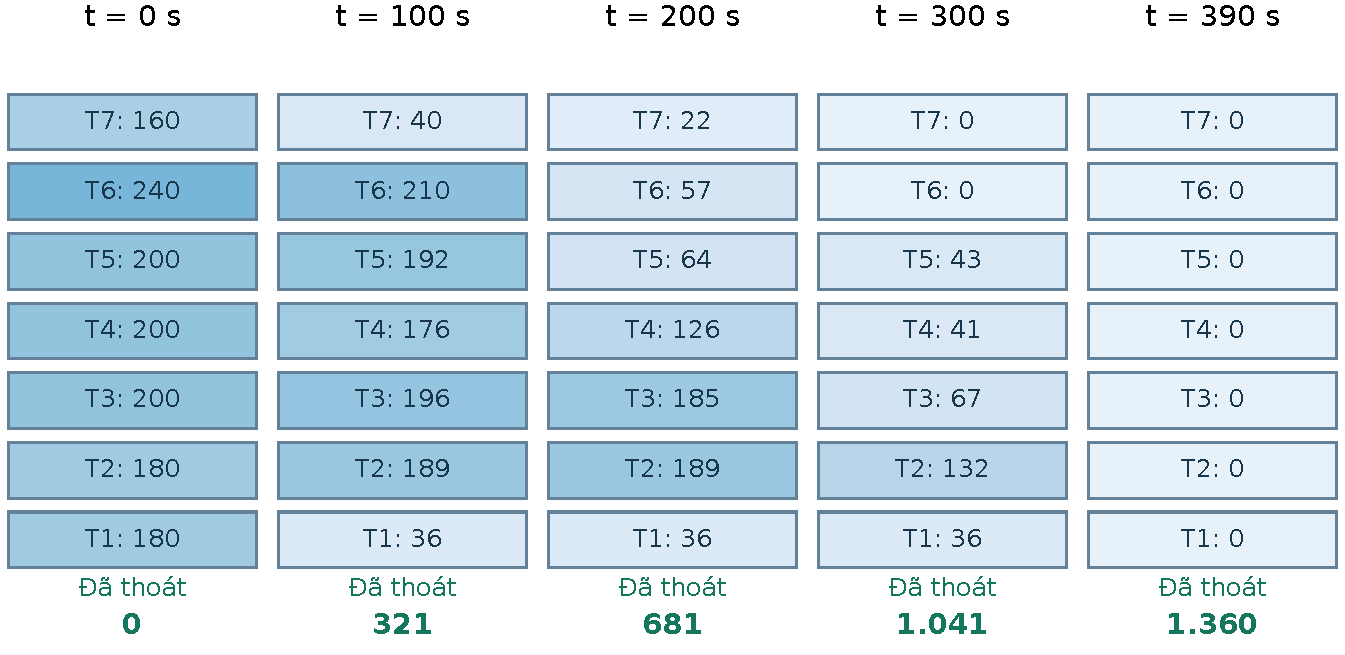
\includegraphics[width=\linewidth]{figures/timeline.pdf}
\caption{Năm khung phát lại giản lược theo tầng của lịch M4 tại 0, 100, 200, 300 và 390 s. Mỗi ô ghi số người còn trong hệ tại một tầng; người đang đi được quy về tầng đầu cạnh. Dòng xanh ghi số đã thoát. Tổng mỗi khung luôn bằng 1.360.}
\label{fig:timeline}\end{figure}
\clearpage\section{THỰC NGHIỆM, KẾT QUẢ VÀ THẢO LUẬN}
\subsection{Thiết lập thực nghiệm và hệ chỉ số}
Thực nghiệm chính gồm bốn phương pháp M1--M4 và bốn kịch bản, tạo thành 16 tổ hợp. Các tổ hợp dùng cùng mặt bằng, dân số đầy tải 1.360 người, bước thời gian 5 s và thời hạn 900 s. Bộ chính được giữ cố định; các thực nghiệm bổ sung về đối chứng, mức tải, thời gian tính toán và độ nhạy được lưu tách biệt.

\begin{table}[htbp]\centering\caption{Các kịch bản trong thiết kế thực nghiệm}
\small\begin{tabularx}{\linewidth}{P{2.8cm}X}\toprule
Kịch bản & Điều kiện nguy cơ\\\midrule
Không sự cố & Không có nguồn cháy, khói hoặc vùng thoát bị khóa.\\
Khói phòng 403 & Khói tại R403 từ 120 s; cháy tại cùng vị trí từ 180 s.\\
Khói cầu thang & Khói tại thang 1 tầng 4 từ 90 s, sau đó lan theo đồ thị nguy cơ.\\
Khóa vùng thoát & Vùng tiếp cận EXIT1 bị khóa từ 120 s; cửa phòng tầng 1 và EXIT2 vẫn mở.\\\bottomrule
\end{tabularx}\end{table}

Lượng thoát và tỷ lệ thoát được đánh giá trước thời gian. Makespan chỉ xác định khi toàn bộ dân số thoát; ``Thoát cuối'' là thời điểm thoát muộn nhất trên tập người đã thoát. Trung bình thời điểm thoát cũng được tính trên tập này. Vì vậy, trung bình của hai phương pháp có lượng thoát khác nhau không được xem là so sánh trên cùng dân số.

\begin{table}[htbp]\centering
\caption[Kết quả 16 tổ hợp phương pháp--kịch bản]{Kết quả 16 tổ hợp. Các cột thời gian tính bằng giây; TB: trung bình thời điểm thoát trên tập đã thoát; Giải: thời gian tính toán bộ giải. Dấu -- ở Hoàn tất nghĩa là còn người chưa thoát. In đậm lượng thoát cao nhất, thời gian tốt nhất trong các phương pháp đạt cùng lượng thoát cao nhất và thời gian giải nhỏ nhất.}
\label{tab:allresults}\small\setlength{\tabcolsep}{3pt}\begin{tabular}{lrrrrrr}
\toprule
PP & Thoát & Tỷ lệ (\%) & Hoàn tất & Thoát cuối & TB & Giải\\\midrule
\multicolumn{7}{l}{\textbf{Không sự cố}}\\
M1 & \textbf{1.360} & \textbf{100,00} & 500 & 500 & 216,30 & \textbf{6,747}\\
M2 & \textbf{1.360} & \textbf{100,00} & 500 & 500 & 216,30 & 11,503\\
M3 & \textbf{1.360} & \textbf{100,00} & 530 & 530 & 231,52 & 46,079\\
M4 & \textbf{1.360} & \textbf{100,00} & \textbf{390} & \textbf{390} & \textbf{199,25} & 94,824\\
\midrule
\multicolumn{7}{l}{\textbf{Khói phòng 403}}\\
M1 & 1.055 & 77,57 & -- & 330 & 159,43 & \textbf{5,222}\\
M2 & 1.217 & 89,49 & -- & 435 & 189,16 & 9,640\\
M3 & 1.212 & 89,12 & -- & 475 & 207,91 & 29,425\\
M4 & \textbf{1.360} & \textbf{100,00} & \textbf{425} & \textbf{425} & \textbf{200,74} & 46,704\\
\midrule
\multicolumn{7}{l}{\textbf{Khói cầu thang}}\\
M1 & 1.070 & 78,68 & -- & 480 & 209,75 & \textbf{2,371}\\
M2 & 1.070 & 78,68 & -- & 480 & 209,75 & 3,193\\
M3 & 1.053 & 77,43 & -- & 535 & 218,58 & 9,726\\
M4 & \textbf{1.248} & \textbf{91,76} & -- & \textbf{530} & \textbf{226,33} & 50,334\\
\midrule
\multicolumn{7}{l}{\textbf{Khóa vùng thoát}}\\
M1 & 1.056 & 77,65 & -- & 500 & 220,39 & \textbf{5,317}\\
M2 & \textbf{1.360} & \textbf{100,00} & \textbf{665} & \textbf{665} & 301,33 & 6,073\\
M3 & 1.359 & 99,93 & -- & 830 & 350,33 & 25,595\\
M4 & \textbf{1.360} & \textbf{100,00} & \textbf{665} & \textbf{665} & \textbf{298,33} & 79,243\\
\midrule
\end{tabular}\end{table}

Các giá trị thời gian giải ở bảng tổng hợp là phép đo đơn của bộ chính, không phải trung bình nhiều lần. Phần đo lặp M4 được báo cáo riêng. Không có phép đo đỉnh bộ nhớ trong đợt chính; các giá trị thiếu không được thay bằng 0 MB.

\topic{Không sự cố: thời gian hoàn tất và phân bổ tải}
\hinh[.98]{safe_comparison.pdf}{Số người thoát tích lũy khi không có sự cố. M1 và M2 trùng nhau, được phân biệt bằng nét liền và nét đứt.}
M4 hoàn tất ở 390 s, so với 500 s của M1 và M2; mức giảm là 22\%. Trung bình thời điểm thoát giảm từ 216,30 s xuống 199,25 s. Khi không có nguy cơ thay đổi, việc tái tính tuyến của M2 trả lại cùng lựa chọn ngắn nhất; hai phương pháp còn dùng cùng thứ tự phục vụ và chính sách đặt chỗ, nên các đường cong trùng nhau trong tổ hợp này.

Trong 1.180 người từ tầng trên, M1 phân bổ 400 người qua thang 1 và 780 người qua thang 2; M4 phân bổ 586 và 594 người. Dân số 180 người tầng 1 thoát tại cửa phòng. Sự phân bố gần cân bằng làm giảm tình trạng một thang còn tải lớn trong khi năng lực thang kia không được khai thác đầy đủ.

Đối chứng M1E chia đều 590 người cho mỗi thang và hoàn tất ở 395 s. Khoảng cách với M4 chỉ còn 5 s, tương ứng khoảng 1,27\% so với M1E. Do đó, ở kịch bản không sự cố, cân bằng tải giải thích phần lớn chênh lệch giữa M1 và M4. Kết quả 22\% không được diễn giải như lợi ích riêng của mọi thành phần tối ưu toàn cục.

\subsubsection{Năng lực thang và cận dưới theo lát cắt}
Mỗi cạnh xuống thang có năng lực
\begin{equation}U_e=\lfloor1{,}5\times1{,}3\times5\rfloor=9\quad\text{người/bước}.\end{equation}
Hai cạnh từ tầng 2 xuống tầng 1 tạo một lát cắt mà toàn bộ 1.180 người tầng trên phải đi qua. Nếu bỏ thời gian tiếp cận và rời thang, cận thô chỉ là $5\lceil1.180/18\rceil=330$ s. Cận này chưa tính thời điểm dòng đầu tiên có thể tới lát cắt.

Gọi $r_i$ là bước khởi hành sớm nhất vào cạnh cắt $i$, $d_i$ là thời lượng cạnh và $s_i$ là thời lượng tự do từ đầu ra đến EXIT. Mọi lịch hoàn tất tại bước $K$ phải thỏa mãn
\begin{equation}N_{\mathrm{trên}}\le\sum_{i=1}^{2}U_i\max\{0,K-r_i-d_i-s_i+1\}.\label{eq:cutbound}\end{equation}
Đường ngắn nhất không hàng đợi cho $r_1=6$, $r_2=7$, $d_i=4$ và $s_i=2$. Tại $K=77$ (385 s), vế phải chỉ bằng $9(66+65)=1.179$, thiếu một suất so với 1.180 người. Tại $K=78$ (390 s), vế phải là 1.197. Vì M4 có lịch khả thi hoàn tất ở 390 s, cận dưới này đồng thời xác nhận thời gian hoàn tất tối ưu của kịch bản không sự cố trong mô hình rời rạc.

\bang{cut_bounds}{Cận dưới theo từng lát cắt ngang giữa hai tầng, không sự cố}
Các cận dùng thời gian tiếp cận sớm nhất và cho phép sử dụng trọn năng lực các bước sau đó, nên mang tính lạc quan. Chúng không giả định mọi nguồn có thể cùng tới thang sớm; điều này bảo đảm chiều của bất đẳng thức cận dưới.

\hinh{stair_heatmap.pdf}{Heatmap năng lực vào cạnh thang của M1 và M4 khi không sự cố. Mỗi ô là lượng khởi hành chia cho 9; trục dọc chỉ tầng và cụm thang.}
Heatmap thể hiện thời điểm từng đoạn thang được sử dụng, bổ sung thông tin mà đường cong tổng không biểu diễn. Phân bố tải cuối cùng gần đều chưa đủ bảo đảm tối ưu; vị trí hàng đợi và thời điểm đưa người vào thang còn ảnh hưởng phần đuôi của lịch. Khoảng cách 5 s giữa M1E và M4 là một ví dụ.

\topic{Khói tại phòng 403: hiệu quả về lượng người thoát}
\hinh[.98]{smoke_comparison.pdf}{Số người thoát tích lũy khi khói phát sinh tại phòng 403; các vạch đứng đánh dấu nguồn khói và cháy.}
M1, M2, M3 và M4 lần lượt đạt 1.055, 1.217, 1.212 và 1.360 người thoát. M4 hoàn tất trong 425 s, tăng 305 người so với M1 và 143 người so với M2. Lượng thoát là chỉ số ưu tiên khi các phương pháp đối chứng chưa hoàn tất.

M2 và M4 cùng biết lịch nguy cơ. M2 cập nhật tuyến ở vị trí hiện tại rồi cam kết từng hành động; M4 phối hợp năng lực trên toàn lịch. Khác biệt nằm ở mức độ điều phối giữa các nguồn, không nằm ở việc chỉ M4 có thông tin nguy cơ tương lai.

Trung bình 159,43 s của M1 nhỏ hơn 200,74 s của M4, nhưng M1 còn 305 người chưa thoát. Tập được tính trung bình của M1 loại các trường hợp chưa thể thoát hoặc thoát muộn nếu được tiếp tục phục vụ. Do đó, nhận xét về thời gian phải đi kèm số người thoát; không thể kết luận M1 tốt hơn chỉ từ trung bình nhỏ hơn.

\topic{Khói tại cầu thang: bị chặn bởi nguy cơ}
\hinh[.98]{stair_block_comparison.pdf}{Số người thoát tích lũy khi nguy cơ lan từ thang 1 tầng 4; đường ngang chỉ tổng dân số 1.360.}
M4 đạt 1.248 người, tương ứng 91,76\%; còn 112 người chưa thoát. M1 và M2 cùng đạt 1.070; M3 đạt 1.053. Thời điểm thoát cuối của M4 là 530 s, nhưng makespan toàn dân số không xác định. Cột Thoát cuối trong bảng tổng hợp tách rõ hai đại lượng này.

M1 và M2 cùng đưa 138 người qua thang 1, 752 qua thang 2 và 180 qua cửa tầng 1. Tuy nhiên, lịch và phân bố nguồn khác nhau: riêng R404, M1 đưa được 17 người còn M2 đưa đủ 40. Trùng chỉ số tổng hợp vì vậy không có nghĩa hai phương pháp chọn cùng tuyến hoặc cùng tập người; thay đổi nguồn được phục vụ vẫn có thể giữ nguyên tổng lưu lượng qua các vùng thoát.

\bang{unserved}{Phân bố 112 người chưa được sơ tán trong lịch M4 khói cầu thang}
Tập còn lại được xác định bằng dân số nguồn trừ tổng số người của các hành trình đã đến EXIT. Theo cách phân rã hiện tại, những người không được gán đường đi tiếp tục ở nguồn; danh tính cá nhân không được mô hình hóa. Bảng mô tả một nghiệm tối ưu về lượng thoát, không khẳng định mọi nghiệm tối ưu phải có cùng phân bố người còn lại theo phòng.

Nguy cơ làm mất các trạng thái hoặc cạnh TEN sau mốc đóng. Đường đi dài hơn chưa chắc tồn tại an toàn; tăng horizon không khôi phục những trạng thái đã bị loại. Đó là cơ chế khiến bộ giải vẫn còn 112 người sau thời hạn 900 s. Chỉ số phơi nhiễm được lưu riêng và không được đồng nhất với thương vong.

\topic{Mất khả năng tiếp cận vùng thoát từ thang tầng 1}
\hinh[.98]{exit_block_comparison.pdf}{Số người thoát tích lũy khi EXIT1 không thể tiếp cận từ 120 s; các cửa tầng 1 và EXIT2 vẫn mở.}
M2 và M4 cùng hoàn tất ở 665 s. Trung bình M4 là 298,33 s, thấp hơn 301,33 s của M2. M1 đạt 1.056; M3 đạt 1.359. Lịch M4 phân bổ 96 người qua thang 1 trước mốc khóa, 1.084 qua thang 2 và 180 qua cửa phòng tầng 1, bảo toàn tổng 1.360.

\subsubsection{Truy vết trường hợp M3 còn một người}
Người chưa thoát của M3 xuất phát từ R405. Lịch ghi nhận người này tới nút thang tầng 1 của cụm 1 ở 95 s, đi sang sảnh lúc 100 s rồi quay lại thang lúc 105 s. Sau đó chỉ còn các hành động chờ đến 900 s. M3 cho phép bước lùi có điểm cục bộ tốt hơn mà không yêu cầu khoảng cách đến EXIT giảm đơn điệu; việc chấm điểm và đặt chỗ không bảo đảm khả thi cho toàn bộ phần đường còn lại.

Khoảng thời gian trước khi EXIT1 đóng bị tiêu hao bởi quyết định cục bộ và hàng đợi. Khi không còn tuyến kịp mốc 120 s, người ở nhánh này không có cạnh đi lên để đổi sang cụm thang kia. Vì vậy, sai khác một người phản ánh một quyết định lịch cụ thể của heuristic, không phải mất dân số do lỗi thống kê. Đây là lý do cần kiểm tra lịch hành động thay vì chỉ so sánh bảng chỉ số.

\topic{Đối chứng bổ sung và chi phí tính toán}
\hinh{aggregate.pdf}{Tổng hợp bộ chính: (a) tỷ lệ thoát; (b) thời gian giải từng tổ hợp. Giá trị được ghi trên cột; đây là phép đo đơn.}
\subsubsection{Đối chứng chia đều hai thang và hệ số M3}
\IfFileExists{tables/balanced.tex}{\bang{balanced}{Đối chứng M1E: tuyến ngắn nhất sau khi chia đều hai thang; dấu -- là chưa hoàn tất}}{}
M1E kiểm soát tác động của chia tải tĩnh, nhưng không cập nhật đích được gán khi nguy cơ xuất hiện. Do đó, kết quả gần M4 trong không sự cố không bảo đảm kết quả tương tự ở ba kịch bản còn lại. Cả ưu thế và hạn chế phải được xét theo từng kịch bản.

\IfFileExists{tables/m3_ablation.tex}{\bang{m3_ablation}{Khảo sát M3 theo hệ số phạt; mỗi ô là số người thoát / thời gian hoàn tất (s), dấu -- là chưa hoàn tất}}{}
Thay đổi hệ số có thể làm thay đổi thứ tự chọn bước, vị trí hàng đợi và số lần đi lùi. Vì vậy, tăng phạt tải không tạo quan hệ đơn điệu với makespan hoặc lượng thoát. Khảo sát này là phép kiểm tra độ nhạy của heuristic, không phải tối ưu siêu tham số trên một tập kiểm định độc lập.

\subsubsection{Đo lặp M4 và thời gian theo giai đoạn}
Các lượt đo bổ sung dùng cùng kịch bản không sự cố, đầy tải, bước 5 s và hạn 900 s. Bộ giải được gọi tuần tự, không bật tracemalloc; các tiến trình nền của máy không được cô lập. Cấu hình máy và số liệu từng lượt được lưu cùng kết quả; thời gian bên dưới không trộn với phép đo đơn của bộ chính.
\IfFileExists{tables/runtime_repeats.tex}{\bang{runtime_repeats}{Các lượt đo M4; $P$ là số pha chi phí, Tăng luồng là số đường tăng trong các pha chi phí}}{}
\IfFileExists{data/runtime_comment.tex}{Máy đo dùng 13th Gen Intel(R) Core(TM) i7-1355U, RAM 15,7 GiB, Windows và Python 3.13.5. Qua 5 lượt, thời gian giải là 150,27 $\pm$ 60,56 s (trung bình và SD mẫu). Các lượt có cùng lượng thoát và thời gian hoàn tất 390 s. Mỗi lượt có 8 phép dò, 74 pha chi phí, 526 lần tăng luồng trong tối ưu chi phí và 3.753 lần tăng trong các phép dò. Độ biến thiên thời gian phản ánh cả điều kiện thực thi trên máy đa dụng; không dùng các phép đo này để suy ra thời gian đáp ứng cố định.
}{}
\IfFileExists{figures/runtime_stages.pdf}{\hinh{runtime_stages.pdf}{Thời gian M4 theo giai đoạn, trung bình trên các lượt đo bổ sung.}}{}
Thời gian dựng mạng gồm các mạng dò và mạng tối ưu cuối. Thời gian dò luồng cực đại bao gồm tất cả phép dò horizon; thời gian luồng chi phí nhỏ nhất gồm các pha đường ngắn nhất và luồng chặn. Phần phân rã và kiểm tra được ghi riêng. Tổng các giai đoạn gần thời gian solver, với sai khác nhỏ do khởi tạo và điều khiển.

\bang{ten}{Quy mô mạng M4 ở giai đoạn tối ưu chi phí của bộ chính}
Horizon dài hơn thường tạo mạng lớn hơn, nhưng số nút cuối chưa giải thích toàn bộ thời gian vì còn các mạng trung gian và số pha. Phiên bản hiện tại dựng mạng độc lập cho mỗi phép dò để duy trì trạng thái dư rõ ràng. Tái sử dụng luồng là hướng cải tiến; việc chuyển giữa horizon có cả tăng và giảm đòi hỏi kiểm soát các phần luồng không còn hợp lệ.

\topic{Độ nhạy toàn tòa nhà và biến thiên mức dân số}
\subsubsection{Bề rộng, tốc độ thang và bước thời gian}
Khảo sát toàn tòa cố định dân số 1.360 và kịch bản không sự cố, với thời hạn 900 s. Mỗi cấu hình thay một yếu tố so với cơ sở: bề rộng thang, tốc độ thang hoặc bước thời gian. Hình học phòng, sức chứa nút và các tham số còn lại được giữ cố định. Đây là các đầu vào tính toán, không phải phương án cải tạo công trình đã được khảo sát.
\IfFileExists{tables/whole_sensitivity.tex}{\bang{whole_sensitivity}{Độ nhạy M4 trên toàn tòa nhà; hàng đầu là cấu hình cơ sở}}{}
Tăng bề rộng làm tăng năng lực vào thang qua phép lấy phần nguyên. Tăng tốc độ làm giảm số bước di chuyển nhưng không trực tiếp tăng năng lực khởi hành. Vì vậy, hai thay đổi tác động lên những ràng buộc khác nhau và không được thay thế cho nhau trong diễn giải.

Trong khoảng khảo sát, bề rộng 1,2--1,8 m cho thời gian hoàn tất 485--335 s, còn tốc độ 0,5--0,9 m/s cho 395--385 s. Chênh lệch cho thấy cấu hình đầy tải nhạy với năng lực vào thang hơn với thời lượng đi tự do trên thang. Với các bước 2, 5 và 10 s, thời gian lần lượt là 440, 390 và 400 s; xu hướng không đơn điệu cần được giải thích qua cả hai phép làm tròn dưới đây.

\subsubsection{Làm tròn năng lực và thời gian}
Với thang cơ sở, năng lực liên tục quy đổi là $1{,}5\times1{,}3\times5=9{,}75$ người/bước; lấy phần nguyên thành 9 làm giảm khoảng $7{,}69\%$. Với cửa, $1{,}2\times1{,}3\times5=7{,}8$ thành 7, giảm khoảng $10{,}26\%$. Mức giảm này đủ lớn để ảnh hưởng các kết luận về thời gian.

Ở bước 2 s, thang cho $\lfloor3{,}9\rfloor=3$ người, tương ứng 1,5 người/s, thấp hơn mức 1,8 người/s của bước 5 s và 1,9 người/s của bước 10 s. Cùng lúc, thời lượng cạnh được làm tròn lên. Do đó, biến thiên theo $\Delta t$ trộn sai số thời lượng và sai số năng lực; không thể xem bước nhỏ hơn là một phép tinh lưới thuần túy của cùng mô hình liên tục. Một mô hình bảo toàn phần lẻ tích lũy cần được triển khai và kiểm chứng riêng.

Khảo sát hệ con tầng 1 được giữ như phép kiểm tra cơ chế cửa, tách khỏi khảo sát toàn tòa:
\bang{sensitivity}{Độ nhạy hệ con 180 người tầng 1; TB tính trên tập đã thoát}
Ở bước 5 s, bề rộng cửa 0,9; 1,2 và 1,5 m cho thời gian hoàn tất 45, 35 và 30 s. Các kết quả này không đại diện cho tác động thay đổi cửa khi hệ thống cầu thang đang chịu tải toàn tòa.

\subsubsection{Mức tải và seed phân bố dân số}
Các mức tải 30\%, 50\% và 70\% tương ứng 408, 680 và 952 người; thời hạn khảo sát là 900 s. Tổng dân số được giữ đúng theo mức tải; seed thay đổi cách phân bổ người vào các nguồn phòng, có chặn theo sức chứa. Các seed từ 2026 đến 2030 tạo năm phân bố ở mỗi mức. Cách làm này khác với nhân đồng đều dân số từng phòng, vốn không sử dụng seed.
\IfFileExists{tables/population.tex}{\bang{population}{Kết quả M4 theo mức tải: trung bình $\pm$ SD mẫu qua các seed phân bố}}{}
SD ở đây mô tả biến thiên do phân bố nguồn, không mô tả bất định của tốc độ, hành vi hay dữ liệu nguy cơ. Các phép đo thời gian mô phỏng không được trộn với thời gian tính toán. Mỗi đầu vào được kiểm tra lịch và bảo toàn dân số trước khi tổng hợp.

\topic{Giới hạn nghiên cứu và kết luận}
\subsubsection{Dữ liệu và miền áp dụng}
Phòng ghép 601-602 có sức chứa 80 người trên chiều dài 9,6 m, còn 705 có 40 người với cùng chiều dài. Đây là hai giá trị trong dữ liệu nguồn theo phân loại khu ghép và phòng đơn, không phải suy ra bằng cùng một định mức diện tích. Nghiên cứu giữ nguyên chúng để truy xuất dữ liệu; cần kiểm tra hồ sơ sử dụng phòng nếu muốn thay bằng dân số thực tế. Chiều sâu 8,8 m và các tọa độ cục bộ không tạo thành một khảo sát ba chiều.

Suất thông hành, tốc độ, độ trễ khói và sức chứa 24/30/36 là tham số minh họa đã phân loại trong bảng cấu hình. Chúng chưa mô tả phản ứng con người, khác biệt khả năng vận động, liều khói hoặc tương tác mật độ liên tục. Nguy cơ là lịch sự kiện biết trước; mô hình chưa đánh giá sai số dự báo hay cảm biến. Chỉ số thoát không được diễn giải thành chỉ số sống sót.

\subsubsection{Thiết kế đối chứng và phép đo}
Các đối chứng dùng đặt chỗ bảo thủ và thứ tự ID cố định. M1E cho thấy cân bằng tải tĩnh đã thu hẹp đáng kể khoảng cách trong không sự cố; khảo sát M3 cho thấy hệ số phạt ảnh hưởng mạnh đến lịch. Kết luận cần gắn với chính sách cụ thể này, không suy rộng thành tính trội đối với mọi heuristic.

Đo lặp trên một máy cung cấp trung bình và SD cho cấu hình hiện tại, nhưng không thay cho đánh giá mở rộng trên nhiều nền tảng. Lịch, số pha và thời gian giai đoạn được lưu để hỗ trợ tái lập. Chưa có đối chiếu OR-Tools hoặc cơ chế tái sử dụng luồng giữa các phép dò; các nội dung đó không được báo cáo như kết quả đã thực hiện.

\subsubsection{Kết luận}
Mô hình tích hợp biểu diễn không gian, nguy cơ và năng lực theo thời gian trong một lịch kiểm chứng được. Với không sự cố, lát cắt cầu thang cho cận dưới 390 s, trùng thời gian của lịch M4. Khi có khói cầu thang, lịch tối ưu lượng thoát còn 112 người được truy xuất theo nguồn. Truy vết trường hợp M3 còn một người cho thấy vai trò của quyết định lùi và mốc đóng trong heuristic cục bộ.

Các kết quả hỗ trợ phân tích thuật toán và nút thắt trong miền giả định đã xác định. Ứng dụng vận hành cần dữ liệu hiện trường, kiểm tra độ phân giải, đánh giá bất định và thẩm định an toàn phù hợp. Những yêu cầu này được tập trung tại đây để phân biệt bằng chứng tính toán với mức độ hiệu chỉnh thực tế của mô hình.
\clearpage\phantomsection\addcontentsline{toc}{section}{Tài liệu tham khảo}
\begingroup\fontsize{12}{17}\selectfont
\begin{thebibliography}{99}\raggedright
\bibitem{map} \emph{Sơ đồ mặt bằng bảy tầng tòa nhà A4: kích thước, cửa ra vào và sức chứa}, tài liệu đầu vào của nghiên cứu, 2026.
\bibitem{code} Lý Thành Đạt, Đinh Đức Mạnh và Phạm Văn Đạt, \emph{Mã nguồn mô hình sơ tán A4 và cấu hình tái lập}, 2026. \href{https://github.com/Datthanhly/Thuattoanungdung}{GitHub: Datthanhly/Thuattoanungdung}. Phiên bản chương trình cơ sở 2.1.0; kho mã nguồn kèm cấu hình, kiểm thử và dữ liệu thực nghiệm tái lập.
\bibitem{ford} L. R. Ford, Jr. và D. R. Fulkerson, ``Constructing Maximal Dynamic Flows from Static Flows,'' \emph{Operations Research}, 6(3), tr. 419--433, 1958. \href{https://doi.org/10.1287/opre.6.3.419}{DOI: 10.1287/opre.6.3.419}.
\bibitem{chalmet} L. G. Chalmet, R. L. Francis và P. B. Saunders, ``Network Models for Building Evacuation,'' \emph{Management Science}, 28(1), tr. 86--105, 1982. \href{https://doi.org/10.1287/mnsc.28.1.86}{DOI: 10.1287/mnsc.28.1.86}.
\bibitem{survey} T. N. Dhamala, ``A survey on models and algorithms for discrete evacuation planning network problems,'' \emph{Journal of Industrial and Management Optimization}, 11(1), tr. 265--289, 2015. \href{https://doi.org/10.3934/jimo.2015.11.265}{DOI: 10.3934/jimo.2015.11.265}.
\bibitem{ahuja} R. K. Ahuja, T. L. Magnanti và J. B. Orlin, \emph{Network Flows: Theory, Algorithms, and Applications}, Prentice Hall, 1993, ISBN 9780136175490. \href{https://www.pearson.com/en-us/subject-catalog/p/P200000003456/9780136175490}{Tài liệu trực tuyến}.
\bibitem{dijkstra} E. W. Dijkstra, ``A note on two problems in connexion with graphs,'' \emph{Numerische Mathematik}, 1, tr. 269--271, 1959. \href{https://doi.org/10.1007/BF01386390}{DOI: 10.1007/BF01386390}.
\bibitem{dinic} E. A. Dinic, ``Algorithm for Solution of a Problem of Maximum Flow in Networks with Power Estimation,'' \emph{Soviet Mathematics Doklady}, 11, tr. 1277--1280, 1970. Thư mục tác giả: \href{https://www.cs.bgu.ac.il/~dinitz/pub.html}{Tài liệu trực tuyến}.
\bibitem{mitflow} D. Karger, \emph{Min Cost Flow}, ghi chú học phần 6.854, MIT, 2021. \href{https://courses.csail.mit.edu/6.854/21/Notes/n10-mincostflow.html}{Tài liệu trực tuyến}.
\bibitem{clrs} T. H. Cormen, C. E. Leiserson, R. L. Rivest và C. Stein, \emph{Introduction to Algorithms}, ấn bản 4, MIT Press, 2022, ISBN 9780262046305. \href{https://mitpress.mit.edu/9780262046305/introduction-to-algorithms/}{Tài liệu trực tuyến}.
\bibitem{networkx} NetworkX Developers, \emph{max\_flow\_min\_cost}, tài liệu chính thức, truy cập 24/10/2026. \href{https://networkx.org/documentation/stable/reference/algorithms/generated/networkx.algorithms.flow.max_flow_min_cost.html}{Tài liệu trực tuyến}.
\bibitem{tracemalloc} Python Software Foundation, \emph{tracemalloc -- Trace memory allocations}, tài liệu chính thức, truy cập 24/10/2026. \href{https://docs.python.org/3/library/tracemalloc.html}{Tài liệu trực tuyến}.
\end{thebibliography}\endgroup
\newcommand{\appendixtables}[1]{%
\setcounter{table}{0}%
\renewcommand{\thetable}{#1.\arabic{table}}%
\renewcommand{\theHtable}{appendix.#1.\arabic{table}}%
}
\clearpage\appendixtables{A}\section*{PHỤ LỤC A. DANH SÁCH KHU PHÒNG}
\addcontentsline{toc}{section}{Phụ lục A. Danh sách khu phòng}
Mỗi dòng biểu diễn một nguồn dân số. Chiều sâu phòng được đặt bằng 8,8 m; sức chứa là giá trị tối đa của dữ liệu mặt bằng. Khu ghép được thống kê một lần để bảo toàn tổng dân số nguồn. Hàng Tổng cộng dân số và số cửa; không cộng các kích thước phòng.
\bang{rooms}{Danh sách 27 khu phòng, tổng sức chứa 1.360 người}

\clearpage\appendixtables{B}\section*{PHỤ LỤC B. KÝ HIỆU}
\addcontentsline{toc}{section}{Phụ lục B. Ký hiệu}
\begingroup\fontsize{12}{16}\selectfont
\begin{longtable}{P{3.5cm}P{10.8cm}}
\caption{Ký hiệu sử dụng trong mô hình và thuật toán}\\
\toprule Ký hiệu & Ý nghĩa\\\midrule\endfirsthead
\multicolumn{2}{l}{\small Bảng B.1 (tiếp)}\\\toprule Ký hiệu & Ý nghĩa\\\midrule\endhead
\bottomrule\endfoot
$G=(V,E)$ & Đồ thị không gian có hướng; $V$ là tập nút, $E$ là tập cạnh.\\
$n,m$ & Số nút và cạnh của đồ thị không gian.\\
$n^{\prime},m^{\prime}$ & Số nút và cạnh thuận của mạng TEN sau cắt trạng thái.\\
$N$ & Tổng dân số nguồn; đầy tải là 1.360 người.\\
$\Delta t,k,K$ & Bước thời gian theo giây, chỉ số bước và horizon theo bước.\\
$\ell_e,v_e$ & Chiều dài cạnh $e$ (m) và tốc độ giả định trên cạnh (m/s).\\
$d_e$ & Số bước đi hết cạnh: $\max(1,\lceil\ell_e/(v_e\Delta t)\rceil)$.\\
$w_e,q$ & Bề rộng sử dụng cạnh (m) và suất thông hành (người/(m.s)).\\
$U_e$ & Năng lực vào cạnh trong một bước, $\lfloor w_eq\Delta t\rfloor$.\\
$C_e$ & Sức chứa cạnh trong cấu hình đoàn: $C_e=d_eU_e$.\\
$B_v$ & Sức chứa của nút $v$ tại một mốc thời gian.\\
$T_v$ & Thời điểm nút mất an toàn, tính theo giây.\\
$x_{e,k}$ & Số người bắt đầu đi trên cạnh $e$ tại bước $k$.\\
$y_{v,k}$ & Số người hiện diện tại nút $v$ sau đến, trước rời ở bước $k$.\\
$z_{v,k}$ & Số người chờ tại $v$ từ bước $k$ sang $k+1$.\\
$\rho_e$ & Tỷ lệ năng lực cạnh đã đặt tại bước khởi hành trong quy tắc M3.\\
$\rho_v$ & Tỷ lệ sức chứa nút đích đã đặt tại bước đến trong quy tắc M3.\\
$\alpha$ & Hệ số phạt của M3, khảo sát các giá trị 1, 2, 4 và 8.\\
$\operatorname{lower}(v)$ & Cận dưới thời gian từ $v$ tới một EXIT theo bước, bỏ qua nguy cơ và hàng đợi.\\
$\operatorname{lower}_{safe}$ & Thời gian đường còn lại có xét mốc nguy cơ, chưa xét hàng đợi.\\
$F(K),F^*$ & Luồng cực đại tới hạn $K$ và lượng thoát tối đa tại hạn cuối.\\
$K^*$ & Horizon nhỏ nhất còn đạt lượng thoát $F^*$.\\
$p(v)$ & Thế đỉnh dùng trong thuật toán luồng chi phí nhỏ nhất.\\
$c^{\prime}(u,v)$ & Chi phí giảm: $c(u,v)+p(u)-p(v)$.\\
$P$ & Số pha đường ngắn nhất thành công trong tối ưu chi phí.\\
$r_i,s_i$ & Thời điểm khởi hành sớm nhất vào cạnh lát cắt $i$ và thời lượng tối thiểu từ đầu ra của cạnh đến EXIT, theo bước.\\
\end{longtable}\endgroup

\clearpage\appendixtables{C}\section*{PHỤ LỤC C. DẤU VẾT DỮ LIỆU VÀ LỊCH}
\addcontentsline{toc}{section}{Phụ lục C. Dấu vết dữ liệu và lịch}
Tệp \texttt{source\_manifest.json} xác định phiên bản mô hình, số nút/cạnh và bộ kết quả. Bảng trình bày 12 ký tự đầu của mã băm SHA-256; chuỗi đầy đủ được lưu trong bản ghi thực nghiệm. Các phương pháp trong cùng kịch bản có chung cấu hình đầu vào, tạo điều kiện đối chiếu có kiểm soát.
\bang{hashes}{Dấu vết đầu vào của các kịch bản chính}
\noindent\textbf{Bản ghi nhóm trích xuất từ lịch M4 không sự cố:}
\lstinputlisting{data/journey_example.json}
Sự kiện thoát của nhóm phòng tầng 1 ở ví dụ trùng bước đến cửa. Các tệp đối chiếu gồm:
\begin{itemize}
\item \texttt{comparison.json} và \texttt{comparison.csv}: 16 bản ghi chỉ số của đợt chính.
\item \texttt{sensitivity.json}: năm cấu hình của hệ con tầng 1.
\item \texttt{assumptions.json}: nguồn và giả định mô hình.
\item \texttt{ground\_floor\_metrics.json}: kết quả hệ con 180 người tầng 1.
\end{itemize}
Các thực nghiệm bổ sung lưu riêng cấu hình, phân bố dân số, kết quả kiểm chứng và lịch nén; các lượt đo lặp lưu chỉ số từng lượt cùng số pha. Kiểm chứng được thực hiện bằng phát lại lịch và tái dựng mức sử dụng tài nguyên. Mã băm phục vụ truy xuất cấu hình; bảng và hình phục vụ trình bày kết quả.

\end{document}
